\documentclass[pageno]{jpaper}

%replace XXX with the submission number you are given from the ASPLOS submission site.
\newcommand{\asplossubmissionnumber}{XXX}

\usepackage[normalem]{ulem}
\usepackage{amsmath,amssymb,amsfonts}
\usepackage{xspace}
\usepackage{xstring}

\usepackage[numbers, sort]{natbib}

\newtheorem{definition}{Definition}
\newtheorem{example}{Example}

\newcommand{\sys}{\mbox{RaceMiner}\xspace}

\newcommand{\figcaption}{% 
	\setlength{\abovecaptionskip}{4pt}%	\setlength{\belowcaptionskip}{1pt}% 
	\caption}

\newcommand{\PP}[1]{
	\vspace{2px}
	\noindent{\bf \IfEndWith{#1}{.}{#1}{#1.}}
}

\begin{document}

\title{
Static Race Detection in OS Kernels by Mining Locking Rules}

\date{}
\maketitle

\thispagestyle{empty}

\begin{abstract}
	
To take advantage of multiple-core architecture of modern CPUs, an operating 
system (OS) is expected to handle concurrency, inevitably introducing many 
concurrent issues. And data race is one of the most harmful concurrent issues 
that can trigger memory or logical bugs. A data race is caused by wrongly 
accessing shared data in different threads. To ensure correct access to shared 
data, fine-grained locking mechanisms are introduced. However, it is hard to 
determine whether a lock should be used for a specific data structure field 
(locking rules) even for an expert developer, due to poor documentation and 
complicated logic of OS code. As a result, OS kernel is prone to data races, 
because necessary locks may be missed by mistake. Static analysis is a common 
technique to help improve code quality, but it is quite challenging to detect 
data races in OS kernels automatically, because of lack of knowledge of locking 
rules and high complexity of concurrent execution.

In this paper, we design a practical static analysis approach named \sys, to 
effectively detect harmful races that can trigger memory or logical bugs in OS 
kernels by mining locking rules. \sys first employs an alias-aware rule mining 
method to automatically deduce locking rules, and detects data races caused by 
violation of these rules. And then performs a lock-usage analysis to filter out 
false positives caused by concurrency. At last, \sys extracts harmful data 
races from all detected data races through a pattern-based estimation. We have 
evaluated \sys on Linux 6.2, and find xxx data races, with a false positive 
rate of xxx. Among these data races, xxx are estimated to be harmful. We have 
reported these harmful bugs to Linux kernel developers, and xxx of them have 
been confirmed.

\end{abstract}

% !TeX spellcheck = en_US
\section{Introduction}
\label{sec_introduction}

To take advantage of multiple-core architecture of modern CPUs, an OS kernel is 
often designed to be highly concurrent. However, concurrent execution can 
inevitably introduce concurrency bugs. Data race is a common kind of 
concurrency bugs that occurs when multiple threads access the same variable 
concurrently and at least one of the accesses is a write. Some data races are 
quite dangerous and can cause serious bugs such as null-pointer dereferences, 
data inconsistency and infinite loops.

To detect data races effectively, some approaches~\cite{Boyapati:OOPSLA02, 
Anderson:PLDI08, Anderson:PLDI09, Zhou:MICRO19, Flanagan:PASTE01, 
Flanagan:PLDI00, Sadowski:PLATEAU14, ClangThreadSafety, Blackshear:OOPSLA18} 
rely on developers to 
supply annotations that describe the locking discipline such as which lock 
protects a specific data structure field, and detect data races by exploiting 
data structure field accesses that violate these disciplines. For example, 
Clang thread safety analysis~\cite{ClangThreadSafety} requires developers to 
label a variable and the lock to protect it with a {\tt GUARDED\_BY} attribute. 
And then detects data races by finding variable accesses that violate the given 
attribute. However, such annotation-based approaches are not suitable for race 
detection in OS kernels, because even an expert developer can not provide 
accurate annotations, due to poor documentation and complicated logic of OS 
codes.

Some static approaches~\cite{Choi:PLDI02, Engler:SOSP03, Voung:FSE07, 
Pratikakis:PLDI06, Naik:PLDI06} employ lockset-based analysis to detect data 
races automatically. They first collect locks that are acquired when a given 
variable is accessed, and then mine locking rules about whether a given 
variable should be protected by a specific lock. At last, they detect data 
races by checking whether variable accesses violate the mined locking rules. 
However, they do not consider alias relations~\cite{Voung:FSE07, Engler:SOSP03} 
or just use imprecise flow-insensitive alias analysis~\cite{Choi:PLDI02, 
Pratikakis:PLDI06, Naik:PLDI06}, and thus can introduce both false positives 
and false negatives.

Dynamic analysis can acquire run-time information such as memory address, and 
thus complex alias analysis can be avoided. Therefore, some 
approaches~\cite{Lochmann:EuroSys19, Lu:SOSP07, Lu:FSE18, Joshi:ASE08, 
Liu:NSDI07} detect data races dynamically to improve precision. They mine 
implicit code rules in softwares by statistically analyzing execution traces, 
and then use the mined rules to detect related bugs. For example, 
LockDoc~\cite{Lochmann:EuroSys19} records accesses to data structure fields and 
lock acquisitions of an instrumented Linux kernel, and then infers locking 
rules from the recorded accesses. After that, LockDoc automatically locates 
data structure fields access that violate the inferred locking rules to detect 
concurrency bugs such as data races. However, dynamic analysis suffers from low 
code coverage, and thus the locking rules inferred through execution traces can 
be imprecise. Besides, dynamic analyses are hard to deploy, because they need 
to run OS kernels with instruments. At last, it is difficult for dynamic 
tools to estimate the harmfulness of a data race, because race conditions are 
hard to trigger by running the checked software~\cite{Fonseca:DSN10, 
Burckhardt:ASPLOS10, Liu:FSE14, Zhou:EASE15}.

In this paper, we design a practical static analysis approach named RaceMiner, 
to automatically detect data races and estimate the harmfulness of these data 
races in OS kernels effectively. RaceMiner consists of three key techniques:

(T1) RaceMiner uses an {\em alias-aware rule mining method} to automatically 
deduce locking rules. We observe that an access to a data structure field is 
often protected by the lock in the same data structure as the accessed field. 
And this relationship between accessed field and the protecting lock can be 
effectively inferred from a special data structure named alias 
graph~\cite{Li:ASPLOS22, Kastrinis:CC18}. Specifically, fields in the same data 
structure have the same ancestor in the alias graph, and thus whether an 
accessed field and a specific lock are in the same data structure can be 
inferred by finding a common ancestor in the alias graph. Moreover, with 
benefits from precise field-sensitive alias relationships of alias graph, 
RaceMiner can accurately extract the accessed field and its corresponding 
protecting lock. After obtaining the accessed field and protecting lock pairs, 
RaceMiner calculates the proportion of field accesses protected by a specific 
lock in all field accesses. If the proportion is larger than a given threshold, 
the accessed field is determined to be protected by the protecting lock.

(T2) RaceMiner uses a {\em lock-usage analysis} to filter out false positives 
caused by concurrency. After mining locking rules, RaceMinder detects data 
races by checking whether a given data structure field access violates the 
locking rules. To reduce false negatives, RaceMinder conservatively assumes 
every two functions can be executed concurrently, and thus can introduce false 
positives. However, we observe that each kernel module has an initialization 
phase, after which many functions can be called concurrently by other modules. 
When performing initialization, the kernel module serially initialized the lock 
and prepare other data for subsequent operations. And thus functions with the 
lock initialization and functions called by them tend not to be executed 
concurrently. Based on this observation, RaceMiner extracts all functions 
reachable from the function with a lock initialization operation such as {\tt 
spin\_lock\_init()}, and suppose that this function can not be executed in 
parallel.

(T3) RaceMiner uses a {\em pattern-based estimation} to extract harmful races 
that can trigger memory or logical bugs such as null-pointer dereferences and 
data inconsistency. Some data races are benign, and developers do not put 
effort into repairing them because they can not cause serious memory or logical 
bugs. Therefore, it is important to estimate the harm a data race can bring. We 
observe that harmful data races can be estimated by given patterns. For 
example, if a raced data performs as an operand of a dereference instruction, a 
null-pointer dereference can occur; if a raced data is accessed for more than 
once and data inconsistency can occur. Based on this observation, RaceMiner 
uses some patterns to extract harmful races that can cause memory or logical 
bugs automatically.

We have implemented RaceMiner with LLVM~\cite{clang} and Z3~\cite{z3}. 
RaceMiner performs automated static analysis on the LLVM bytecode of the 
checked OS kernel. Overall, we make three main contributions in this paper:

\begin{itemize}
	\item We analyze the challenges of data race detection in OS kernels, and 
	propose three key techniques to address	these challenges: (T1) an {\em 
	alias-aware rule mining method} to automatically deduce locking rules; (T2) 
	a {\em lock-usage analysis} to filter out false positives caused by 
	concurrency; (T3) a {\em pattern-based estimation} to extract harmful data 
	races that can trigger memory or logical bugs such as null-pointer 
	dereferences and data inconsistency.
	\item Based on these three key techniques, we design a practical static 
	analysis approach named RaceMiner, to effectively detect data races and 
	estimate the harmfulness of these data races in OS kernels.
	\item We have evaluated RaceMiner on Linux 6.2, and find xxx data races, 	
	with a false positive rate of xxx. Among these data races, xxx are 
	estimated to be harmful. We have reported these harmful bugs to Linux 
	kernel developers, and xxx of them have been confirmed.
\end{itemize}

The rest of this paper is organized as follows. Section~\ref{sec_motivation} 
introduces the motivation and challenges of data race detection in OS kernels. 
Section~\ref{sec_technique} introduces our key techniques to address these 
challenges. Section~\ref{sec_framework} introduces RaceMiner. 
Section~\ref{sec_evaluation} shows our evaluation. Section~\ref{sec_discussion} 
makes a discussion about RaceMiner. Section~\ref{sec_related} presents related 
work, and Section~\ref{sec_conclusion} concludes this paper.
% !TeX spellcheck = en_US
\section{Background and Motivation}
\label{sec_motivation}

\subsection{A Motivating Example}
\label{subsec_motivating_example}

\begin{figure}[htbp]
	\centering
	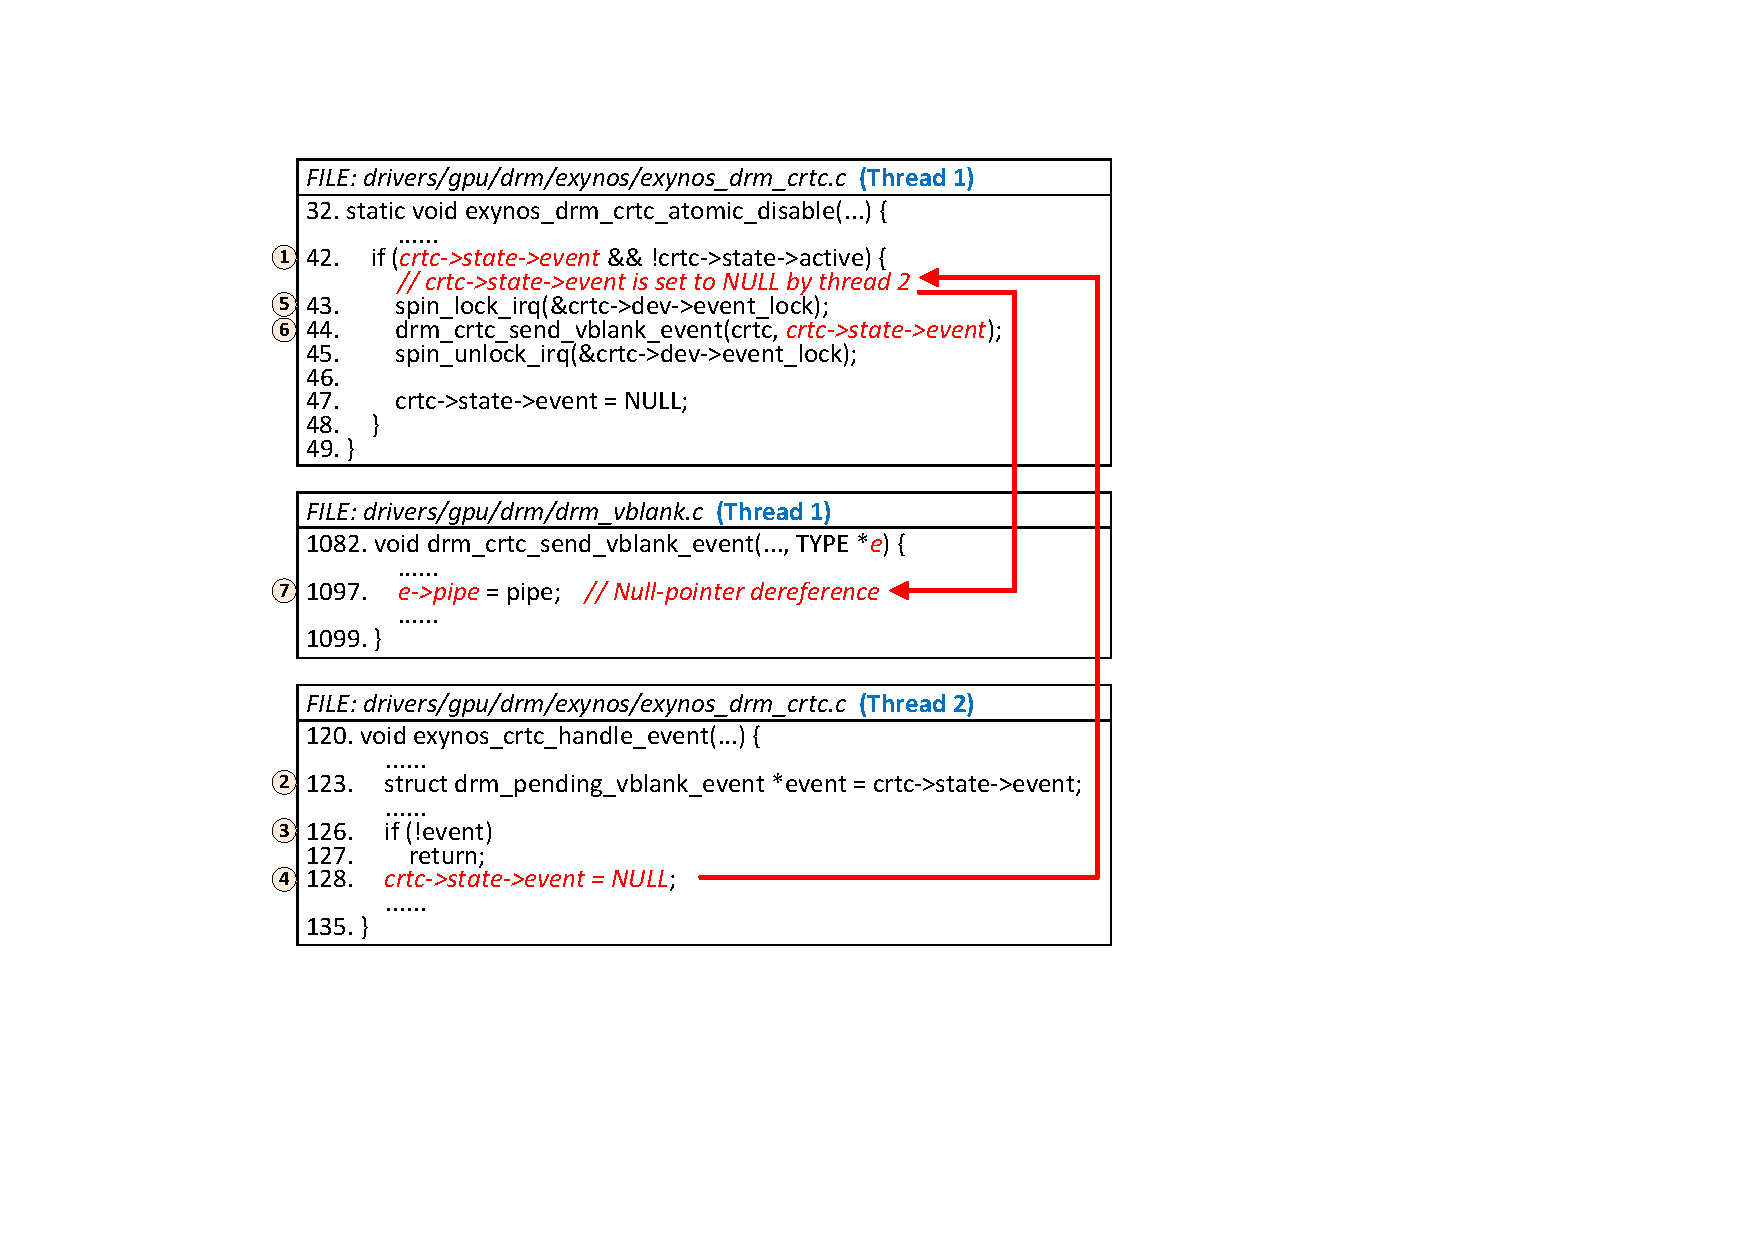
\includegraphics[width=1\linewidth]{figures/fig_bug_demo.pdf}
	\figcaption{A null-pointer dereference due to data race in Linux 6.2.}
	\label{fig_bug_demo}
\end{figure}
Figure~\ref{fig_bug_demo} shows a real null-pointer dereference caused by a 
data race in the Linux DRM driver. In the DRM driver, the functions {\tt 
exynos\_drm\_crtc\_atomic\_disable()} and {\tt exynos\_crtc\_handle\_event()} 
can execute concurrently. We exploit \textcircled{\footnotesize{n}} to 
represent the execution order of instructions and show one execution case in 
the left of Figure~\ref{fig_bug_demo}. In Thread 1, the variables {\tt 
crtc->state->event} and {\tt crtc->state->active} is checked by an if statement 
in the function {\tt exynos\_drm\_crtc\_atomic\_disable()}. After the condition 
is calculated to be true, the function {\tt exynos\_crtc\_handle\_event()} is 
executed in Thread 2. In this function, the value of {\tt crtc->state->active} 
is assigned to {\tt event} (\textcircled{\footnotesize{2}}) and then {\tt 
event} is checked in an if statement (\textcircled{\footnotesize{3}}). If it is 
not NULL, the variable {\tt crtc->state->event} is assigned with NULL 
(\textcircled{\footnotesize{4}}). Right after this assignment, the function 
{\tt drm\_crtc\_send\_vblank\_event} is called  in Thread 1 
(\textcircled{\footnotesize{6}}) with the argument {\tt crtc->state->active}, 
after acquiring the lock {\tt crtc->dev->event\_lock} 
(\textcircled{\footnotesize{5}}). In the called function, the variable {\tt 
crtc->state->event} is dereferenced through {\tt e->pipe} 
(\textcircled{\footnotesize{6}}). In this execution case, the data structure 
{\tt crtc->state->event} is first assigned with NULL and then dereferenced, and 
thus a null-pointer dereference can occur.

This bug is triggered only when {\tt crtc->state->event} is set to NULL by 
Thread 2 right after the first condition of the if statement in Thread 1 is 
calculated to be true. Such requirement is difficult to satisfy by executing 
existing test suites. In fact, this bug had existed for nearly 6 years since 
Linux 4.14 (Released in Nov. 2017), and it was fixed by us based on a report 
generated by \sys. 
 
\subsection{Challenges}
\label{subsec_challenges}
Detecting data races and estimating their harmfulness in OS kernels have three 
main challenges:

\PP{C1: Getting locking rules.} The relationship between variables and locks 
are not well documented in OS kernels, making it hard to determine whether a 
specific variable should be protected by a lock and which lock is 
required (locking rules), even for an expert developer. And thus existing 
annotation-based approaches~\cite{Boyapati:OOPSLA02, Anderson:PLDI08, 
Anderson:PLDI09, Zhou:MICRO19, Flanagan:PASTE01, Flanagan:PLDI00, 
Sadowski:PLATEAU14, ClangThreadSafety, Blackshear:OOPSLA18} are difficult to 
apply to race detection in OS kernels. Other approaches~\cite{Choi:PLDI02, 
Engler:SOSP03, Voung:FSE07, Pratikakis:PLDI06, Naik:PLDI06} employ 
lockset-based analysis to detect data races automatically, but they do not 
consider alias relations~\cite{Voung:FSE07, Engler:SOSP03} or just use 
imprecise flow-insensitive alias analysis~\cite{Choi:PLDI02, 	
Pratikakis:PLDI06, Naik:PLDI06}. However, due to the heavy use of pointers and 
data structure fields in OS code, the alias relationships between variables can 
be very complex, and thus lacking effective alias analysis can introduce many 
false locking rules.

\PP{C2: Dropping false data races.} Static analysis suffers from false 
positives. For example, each data race involves more than one code paths that 
should be able to concurrently execute. However, which code can execute 
concurrently is not well documented for an OS kernel, and it is also hard to 
determine concurrent code statically due to the complexity of OS code. Thus 
static analysis can report many false data races.

\PP{C3: Estimating harmfulness of data races.} Many data races are benign, and 
can not cause memory or logic bugs, and thus developers are unwilling to put 
effort into repairing them. To automatically detect harmful data races, most 
approaches~\cite{Narayanasamy:PLDI07, Sen:PLDI08, Kasikci:SOSP13, 
Kasikci:ASPLOS12} estimate harmfulness of data races through dynamic analysis, 
and explore thread interleavings to trigger data races to estimate their 
harmfulness. However, they suffer from low code coverage and thus can miss many 
real harmful data races.



% !TeX spellcheck = en_US
\section{Race Detection by Mining Locking Rules}
\label{sec_technique}
To address the above challenges, we propose three key techniques. For {\em C1}, 
we propose an {\em alias-aware rule mining method} to automatically deduce 
locking rules. For {\em C2}, we propose a {\em lock-usage analysis} to filter 
out false data races by validating the concurrency of kernel code. For {\em 
C3}, we propose a pattern-based estimation to extract harmful races that can 
trigger memory or logical bugs such as null-pointer dereference and data 
inconsistency. We introduce them as follows:

\subsection{Alias-Aware Rule Mining Method}
\label{subsec_rule_mining}
The relationship between variables and locks is not well documented in OS 
kernels, but it can be inferred from the kernel code. Specifically, a variable 
is often protected by the lock stored in the same data structure. And thus if a 
variable is accessed after acquiring a lock existing in the same data structure 
in most cases, it is likely to be protected by the lock. Whether a variable and 
the protecting lock exist in the same data structure can be determined through 
an alias graph~\cite{Li:ASPLOS22, Kastrinis:CC18} by finding their common 
ancestor. Based on this insight, we propose an {\em alias-aware rule mining 
method} to deduce locking rules automatically. Moreover, with benefits from 
precise field-sensitive alias relationships of alias graph, our alias-aware 
rule mining method can find data structure filed and its protecting lock 
effectively.

\PP{Alias Graph.} It is an important data structure to infer relationship 
between variable and its protecting lock in our analysis, so we introduce it 
and its update first. 

An alias graph is a 2-tuple $\mathit{G = \left<N, E\right>}$, where 
$\mathit{N}$ is a set of nodes, and each node $\mathit{n}$ represents an alias 
set that points to one abstract object. $\mathit{E}$ is a set of labeled edges. 
Each edge is labeled with a data structure field or a dereference operator 
``$\mathit{*}$'', which represents how an abstract object is accessed. In an 
alias node, a variable residing in a node followed by a sequence of edge
labels forms an access path~\cite{Kastrinis:CC18, Cheng:PLDI00}. In this paper, 
we replace the variable in an access path with its structure name to represent 
a data structure field.

An alias graph is updated by handling four types of instructions that  
change alias relationships: MOVE($\mathit{v_1 = v_2}$), STORE ($\mathit{*v_2 = 
v_1}$), LOAD ($\mathit{v_1 = *v_2}$) and GEP ({$\mathit{v_1 = \&v_1->f}$}). We 
exploit {$\mathit{n_x}$} to represent the node whose representing alias set 
includes $\mathit{v_x}$, and introduce how the four types of instructions 
update alias graphs. For a MOVE operation, $\mathit{v_1}$ is moved from 
$\mathit{n_1}$ to $\mathit{n_2}$. After this operation, $\mathit{v_1}$ and  
$\mathit{v_2}$ are represented by the same node, which indicates they become 
aliases. For a STORE operation, the existing outgoing edge from $\mathit{n_2}$ 
is dropped first, and then a new edge labeled with $\mathit{*}$ from 
$\mathit{n_2}$ to $\mathit{n_1}$ is inserted. After this operation, 
$\mathit{v_1}$ and $\mathit{*v_2}$ are represented by the same node, which 
indicates they become aliases. For a LOAD operation, the analysis first finds 
the destination node of the edge that comes from $\mathit{n_2}$ and is labeled 
with $\mathit{*}$, and then moves $\mathit{v_1}$ to the destination node. And 
after this operation, $\mathit{v_1}$ and $\mathit{*v_2}$ are represented by the 
same node, which indicates they become aliases. GEP operation is similar to 
LOAD, expect that the edge is labeled with a data structure field $\mathit{f}$, 
instead of a dereference operator $\mathit{*}$.

\begin{figure}[htbp]
	\centering
	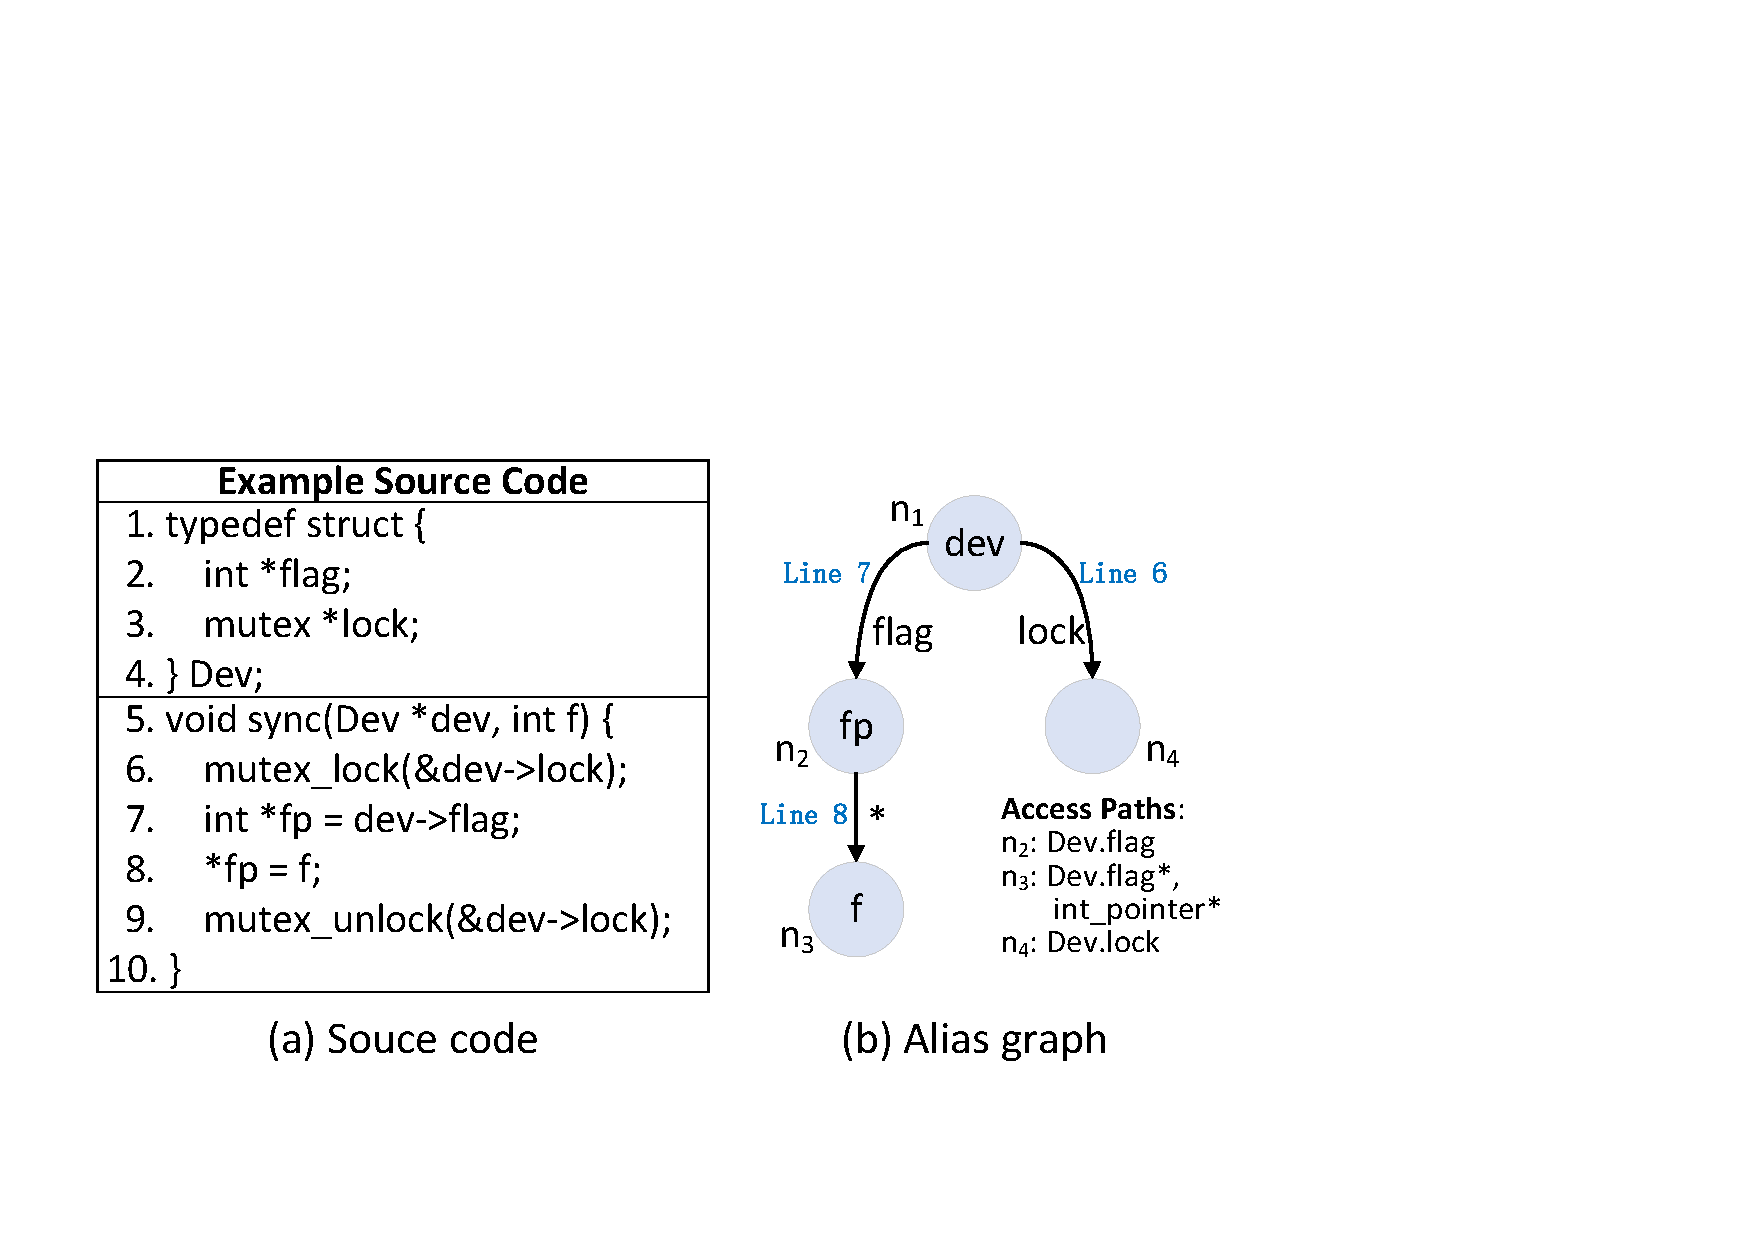
\includegraphics[width=0.9\linewidth]{figures/fig_demo_alias_graph.pdf}
	\figcaption{Example of alias graph.}
	\label{fig_demo_alias_graph}
\end{figure}

\noindent{\textbf{\em Example.}} Figure~\ref{fig_demo_alias_graph} shows a 
piece of driver-like source code and its alias graph. In this example, after a 
GEP (\&dev->lock) operation at Line 6, an edge labeled with {\tt lock} from 
node $\mathit{n_1}$ to node $\mathit{n_4}$ is inserted. Similarly, an edge 
labeled with {\tt flag} from node $\mathit{n_1}$ to node $\mathit{n_2}$ is 
inserted after Line 7. At last, an edge labeled with a dereference operator 
($\mathit{*}$) is inserted after the STORE (*fp = f) operation at Line 8. The 
final alias graph is shown in Figure~\ref{fig_demo_alias_graph}(b), and access 
paths are shown in the bottom left corner. Take node $\mathit{n_3}$ as an 
example, it can represent two fields, one is {\tt Dev.flag*}, and the other is 
{\tt int\_pointer*} (we exploit int\_pointer to represent a pointer points to 
an integer, and regard it as a data structure for convenience). 

\begin{figure}[htbp]
	\centering
	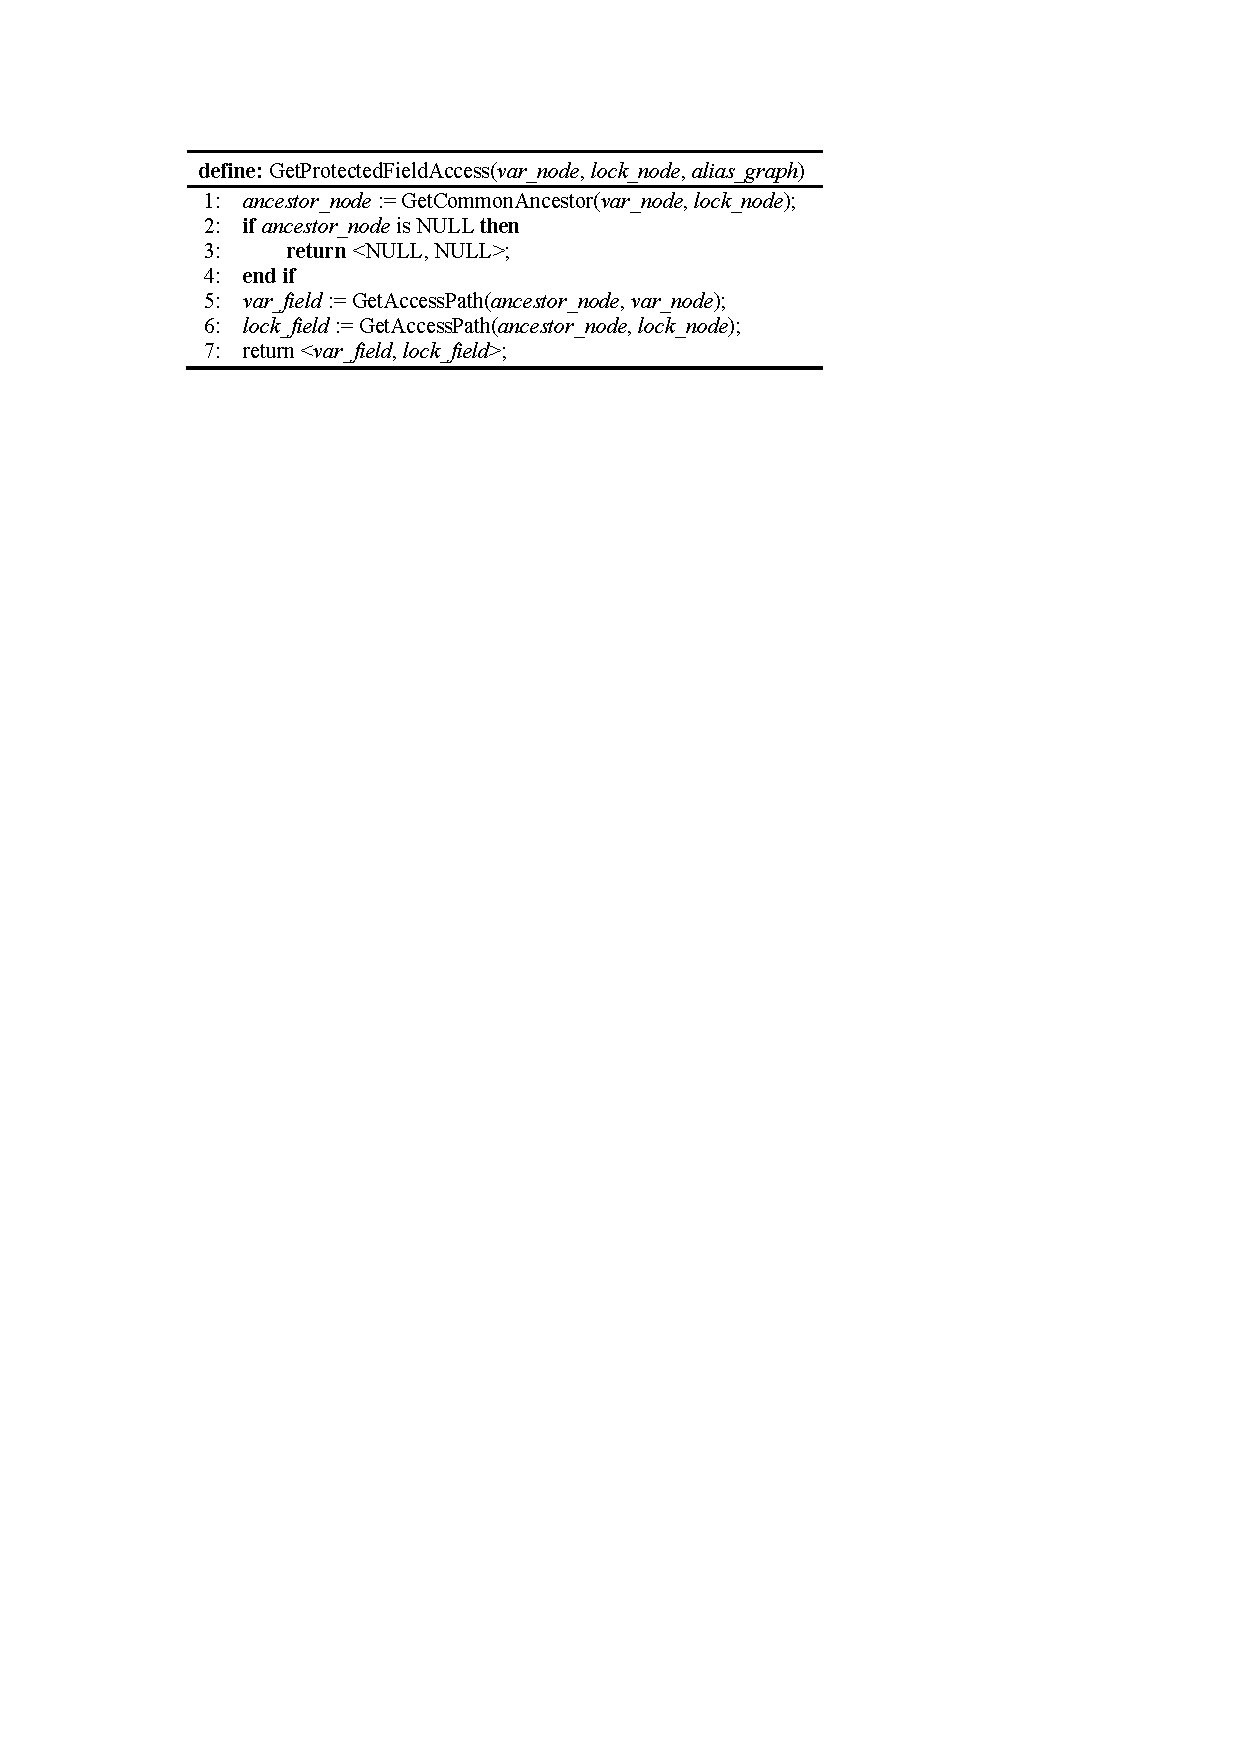
\includegraphics[width=1\linewidth]{figures/fig_pseudocode_get_access.pdf}
	\figcaption{Pseudocodes to get accessed field and protecting lock.}
	\label{fig_pseudocode_get_access}
\end{figure}

Given an alias graph, whether a variable and a lock exist in the same data 
structure can be determined by finding a common ancestor. If they are in the 
same data structure, the lock is likely to protect the variable when it is 
accessed. Figure~\ref{fig_pseudocode_get_access} shows the pseudocode to 
get the field of the accessed variable and the field of the protecting lock in 
the form of access path, if they exist in the same data structure. Given a node 
of an accessed variable and a node of a lock variable, the analysis first gets 
the common ancestor of the two nodes (Line 1). And then, if the common ancestor 
does not exist, the analysis returns a NULL pair (Lines 2-3). Otherwise, the 
analysis gets the access path for the node of the accessed variable and the 
node of the lock variable from the common ancestor (Lines 5-7).

Take the alias graph in Figure~\ref{fig_demo_alias_graph} as an example, {\tt 
\&dev->flag} is represented by node $\mathit{n_2}$, and {\tt \&dev->lock} is 
represented by node $\mathit{n_4}$. The two nodes have a common ancestor 
$\mathit{n_1}$, and thus the accessed variable {\tt \&dev->flag} and the 
protecting lock {\tt \&dev->lock} can be inferred to exist in the same data 
structure (namely {\tt Dev}). Therefore, the structure field Dev.flag is likely 
to be protected by the lock stored in the structure field Dev.lock.

\begin{figure}[htbp]
	\centering
	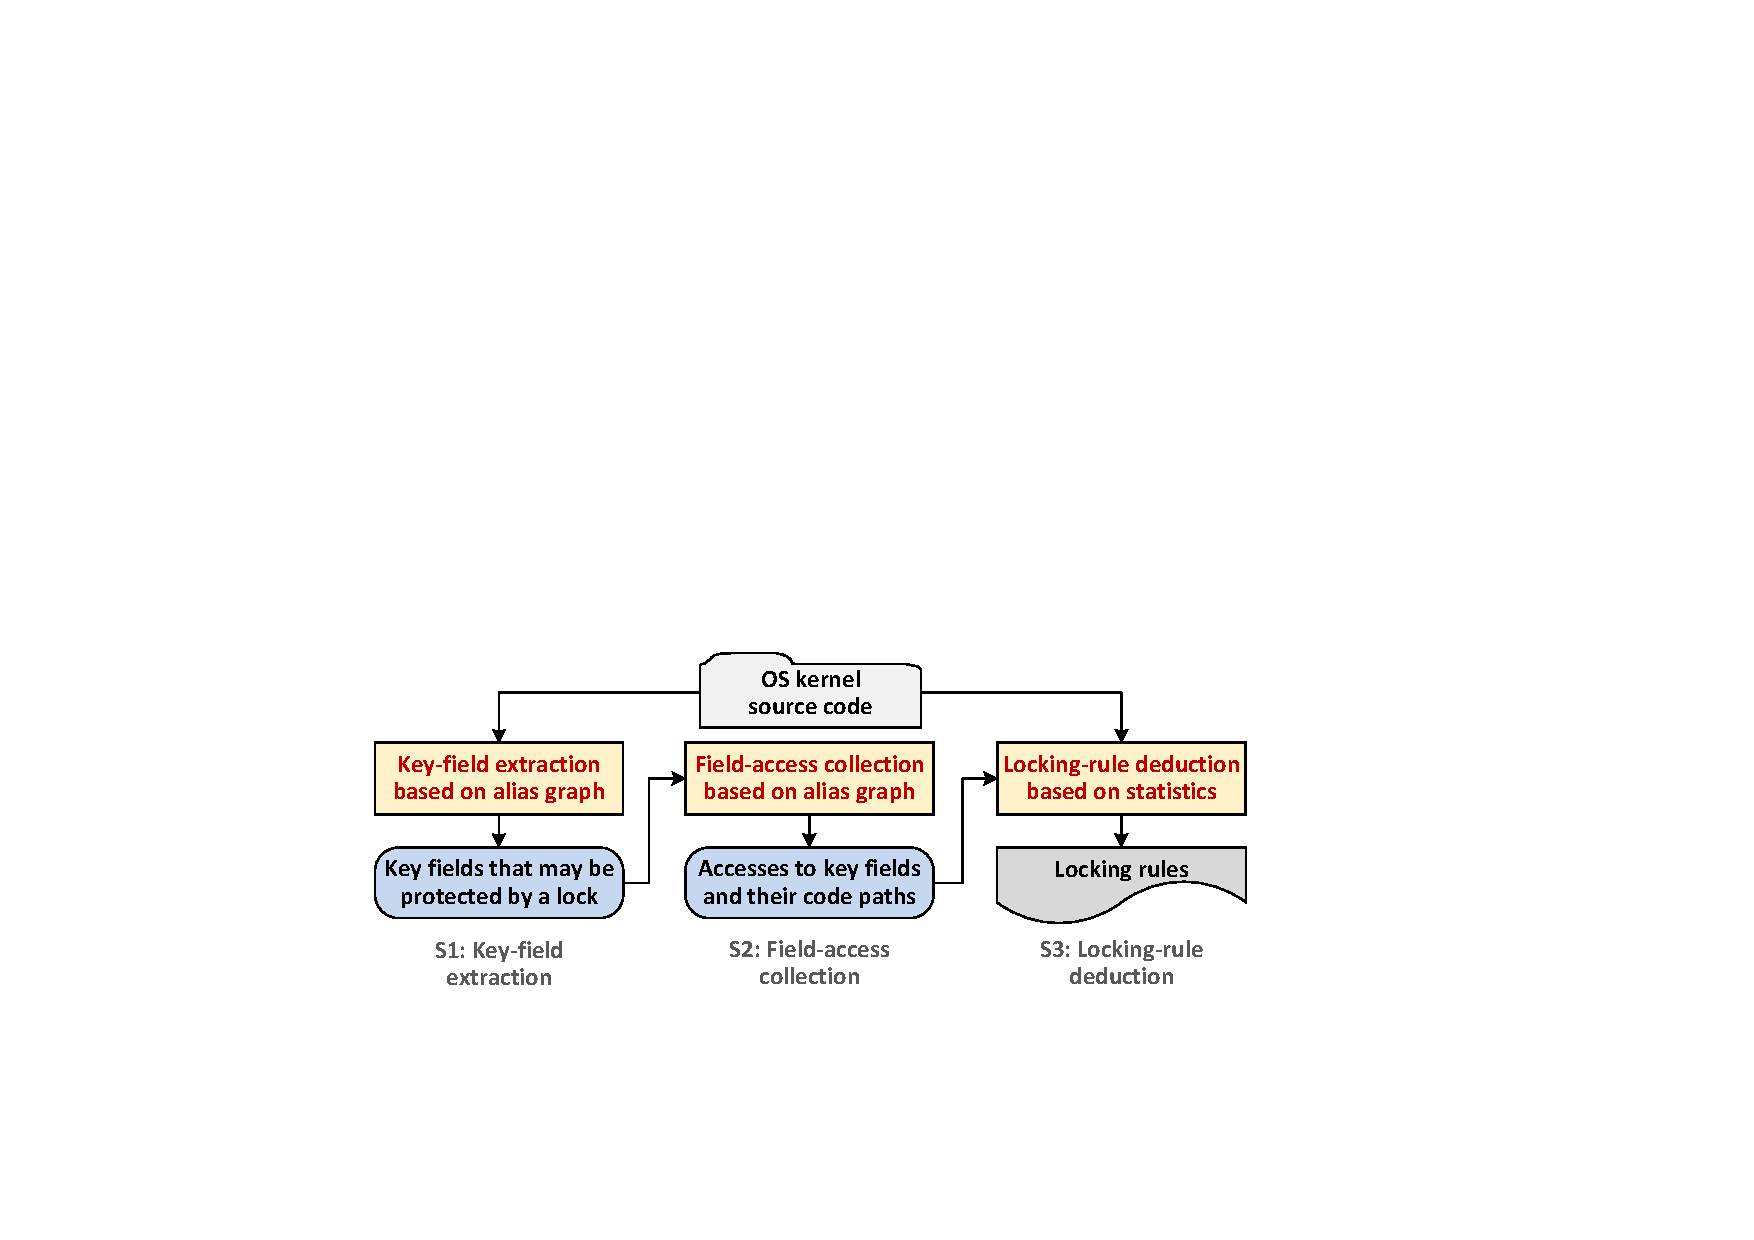
\includegraphics[width=1\linewidth]{figures/fig_workflow.pdf}
	\figcaption{Workflow of locking-rule mining.}
	\label{fig_workflow}
\end{figure}

Based on the alias graph, our alias-aware rule mining method performs an 
inter-procedural path-based~\cite{Li:ASPLOS22}, field-sensitive and alias-aware 
analysis to effectively mine locking rules about whether a specific variable 
should be protected by a lock and which lock is required. Overall, our 
alias-aware rule mining method has three main stages shown in 
Figure~\ref{fig_workflow}. In Stage 1, it extracts key variables that may be 
protected by a lock. In Stage 2, it collects all accesses to key fields as well 
as code paths these accesses exist in. In Stage 3, it deduces locking rules by 
calculating the proportion of field accesses protected by a specific lock in 
all field accesses. 

\PP{S1: Key-field extraction.} The OS Kernel has a large code base with 
numerous variables. However, only a small part of variables should be protected 
by a specific lock, and thus collecting all variable accesses can introduce 
much unnecessary overhead. Generally, only a few field accesses can miss 
necessary protecting locks, due to the carelessness of developers. Based on 
this insight, our analysis first extracts key fields that may need to be 
protected by a specific lock, by performing a lock-set analysis to find whether 
a given variable is accessed after acquiring a lock in the same data structure 
as the accessed field in any code path.

\begin{figure}[htbp]
	\centering
	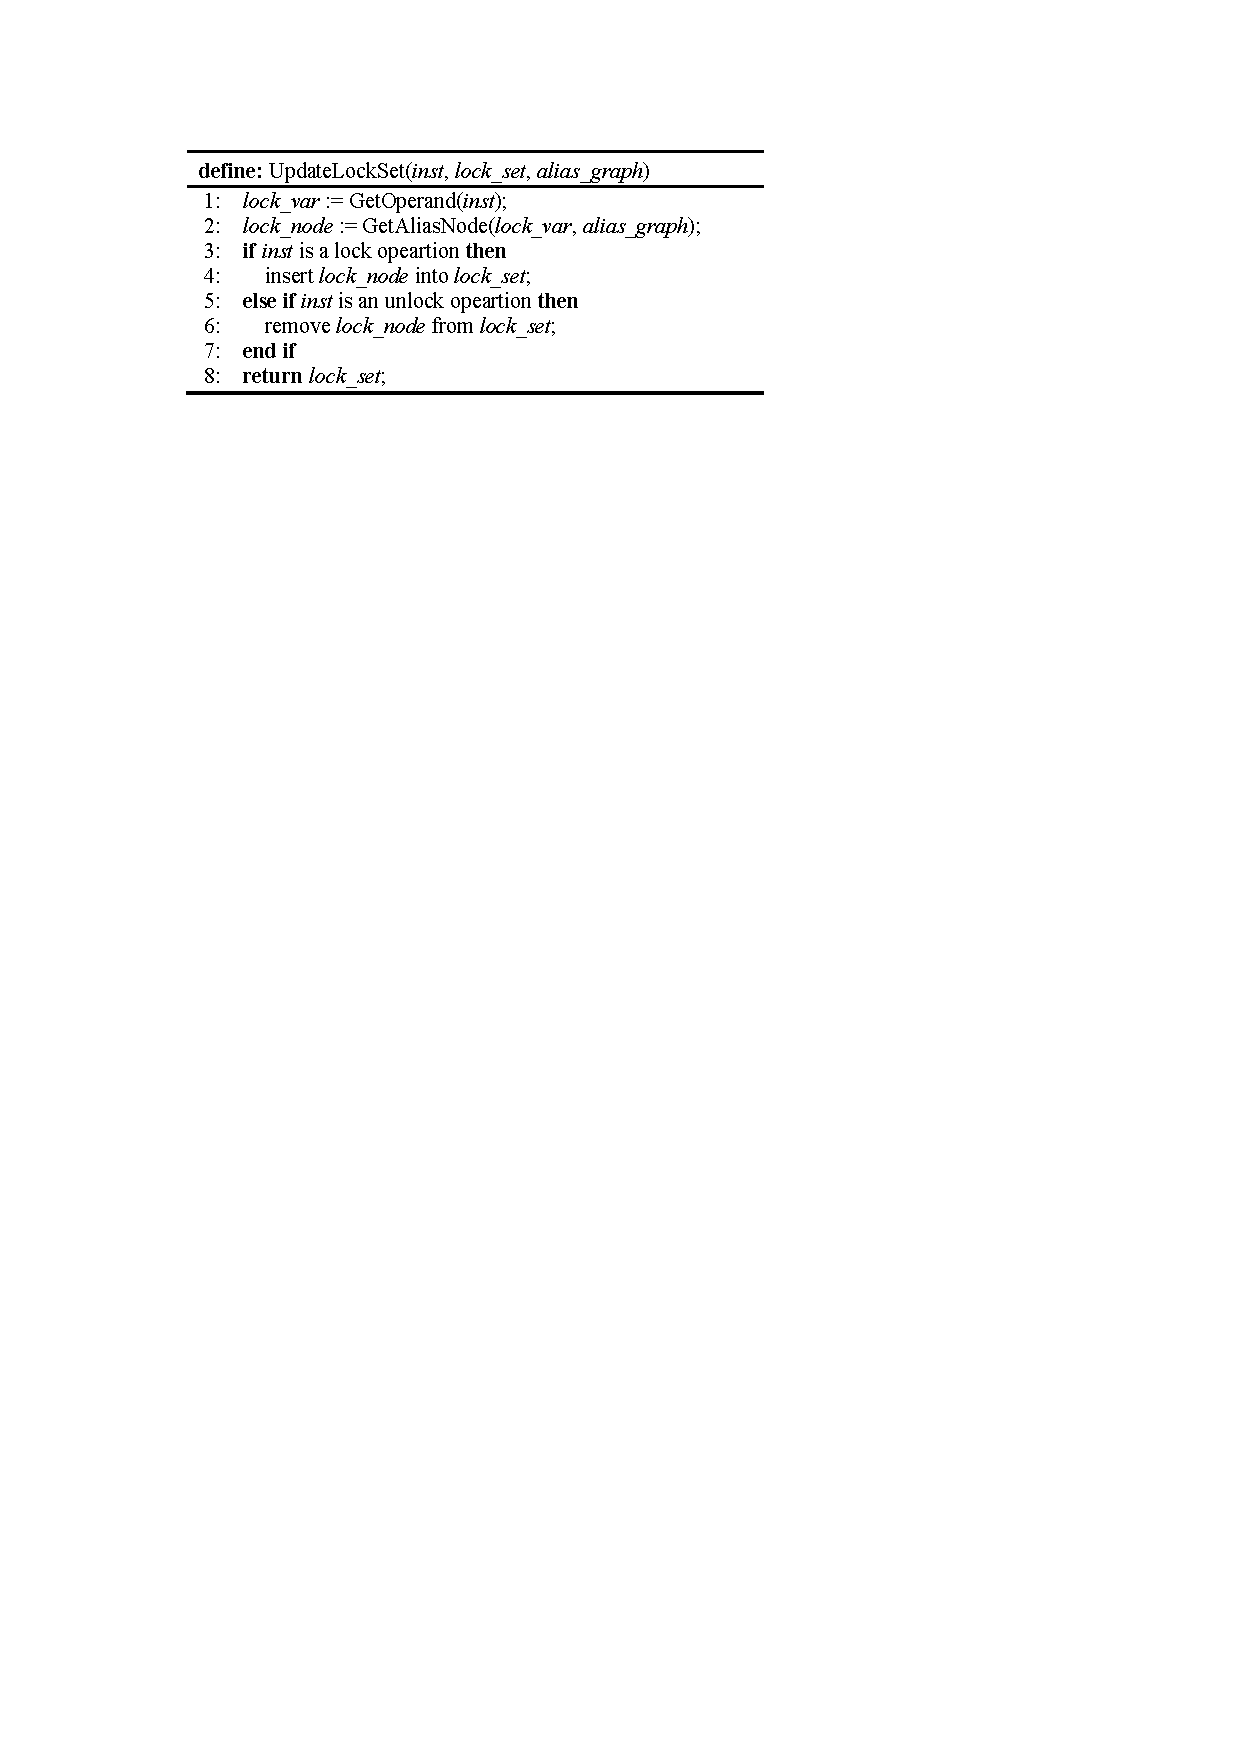
\includegraphics[width=0.9\linewidth]{figures/fig_pseudocode_lock_set.pdf}
	\figcaption{Pseudocodes of lock-set analysis.}
	\label{fig_pseudocode_lock_set}
\end{figure}

Figure~\ref{fig_pseudocode_lock_set} shows the lock-set analysis based on alias 
graph. The analysis first gets the operand of the instruction (Line 1), and 
then gets the node of the operand from the alias graph (Line 2). If the 
instruction is a lock operation, the node of the operand is inserted into the 
lock set (Lines 3-4). Otherwise, if the instruction is an unlock operation, the 
node of the operand is removed from the lock set (Lines 5-6).

\begin{figure}[htbp]
	\centering
	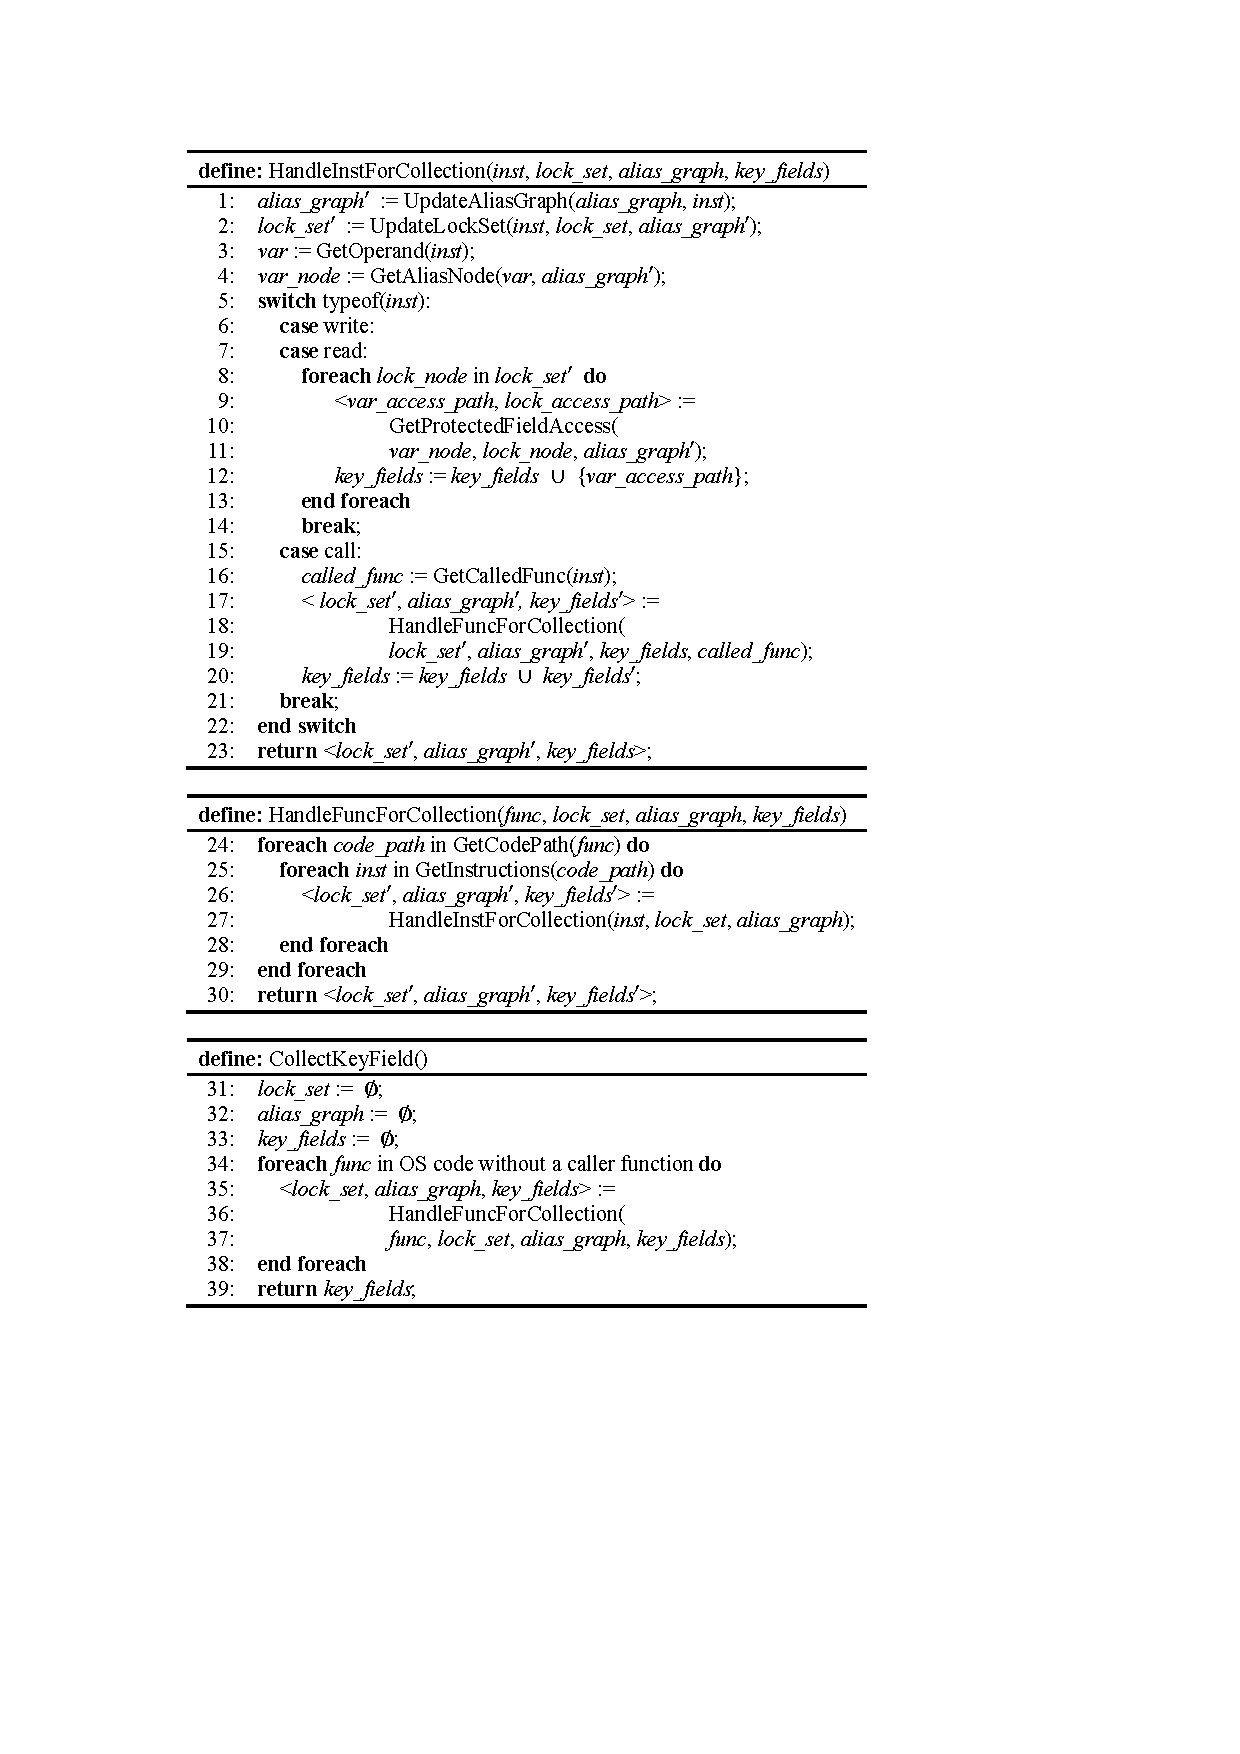
\includegraphics[width=1\linewidth]{figures/fig_pseudocode_field_extract.pdf}
	\figcaption{Pseudocodes of key-field extraction.}
	\label{fig_pseudocode_field_extract}
\end{figure}

Figure~\ref{fig_pseudocode_field_extract} shows the pseudocode to extract key 
fields that may be protected by a specific lock, based on lock-set analysis and 
the alias graph. The analysis starts from each function without a caller 
function (Lines 16-26) and performs a path-based analysis~\cite{Li:ASPLOS22} 
(Lines 17-25). For each instruction in the code path, the analysis first update 
the alias graph according to the instruction with the four operations (MOVE, 
STORE, LOAD and GEP) (Line 1), and then performs a lock-set analysis (Line 2) 
to get all acquired locks. After updating the alias graph and the lock set, if 
the instruction is a write or a read, the analysis first gets the node of the 
operand with the new alias graph (Lines 4-5). And then, for each node of the 
lock variable in the lock set, the analysis uses the alias graph to extract the 
protected data structure field (Lines 6-12). If the field is not NULL, it is 
inserted into the set of key fields (Lines 9-11). For inter-procedural 
analysis, the analysis copies function definition into its call sites, but this 
operation is not shown in Figure~\ref{fig_pseudocode_field_extract} for 
convenience. 

\PP{S2: Field-access collection.} With the key fields extracted in Stage 1, the 
analysis only needs to collect accesses to the variables that are protected in 
some cases, because if a variable is never protected by any lock when is 
accessed, it is less likely to be shared by different threads, and thus can not 
introduce any concurrency issue.

\begin{figure}[htbp]
	\centering
	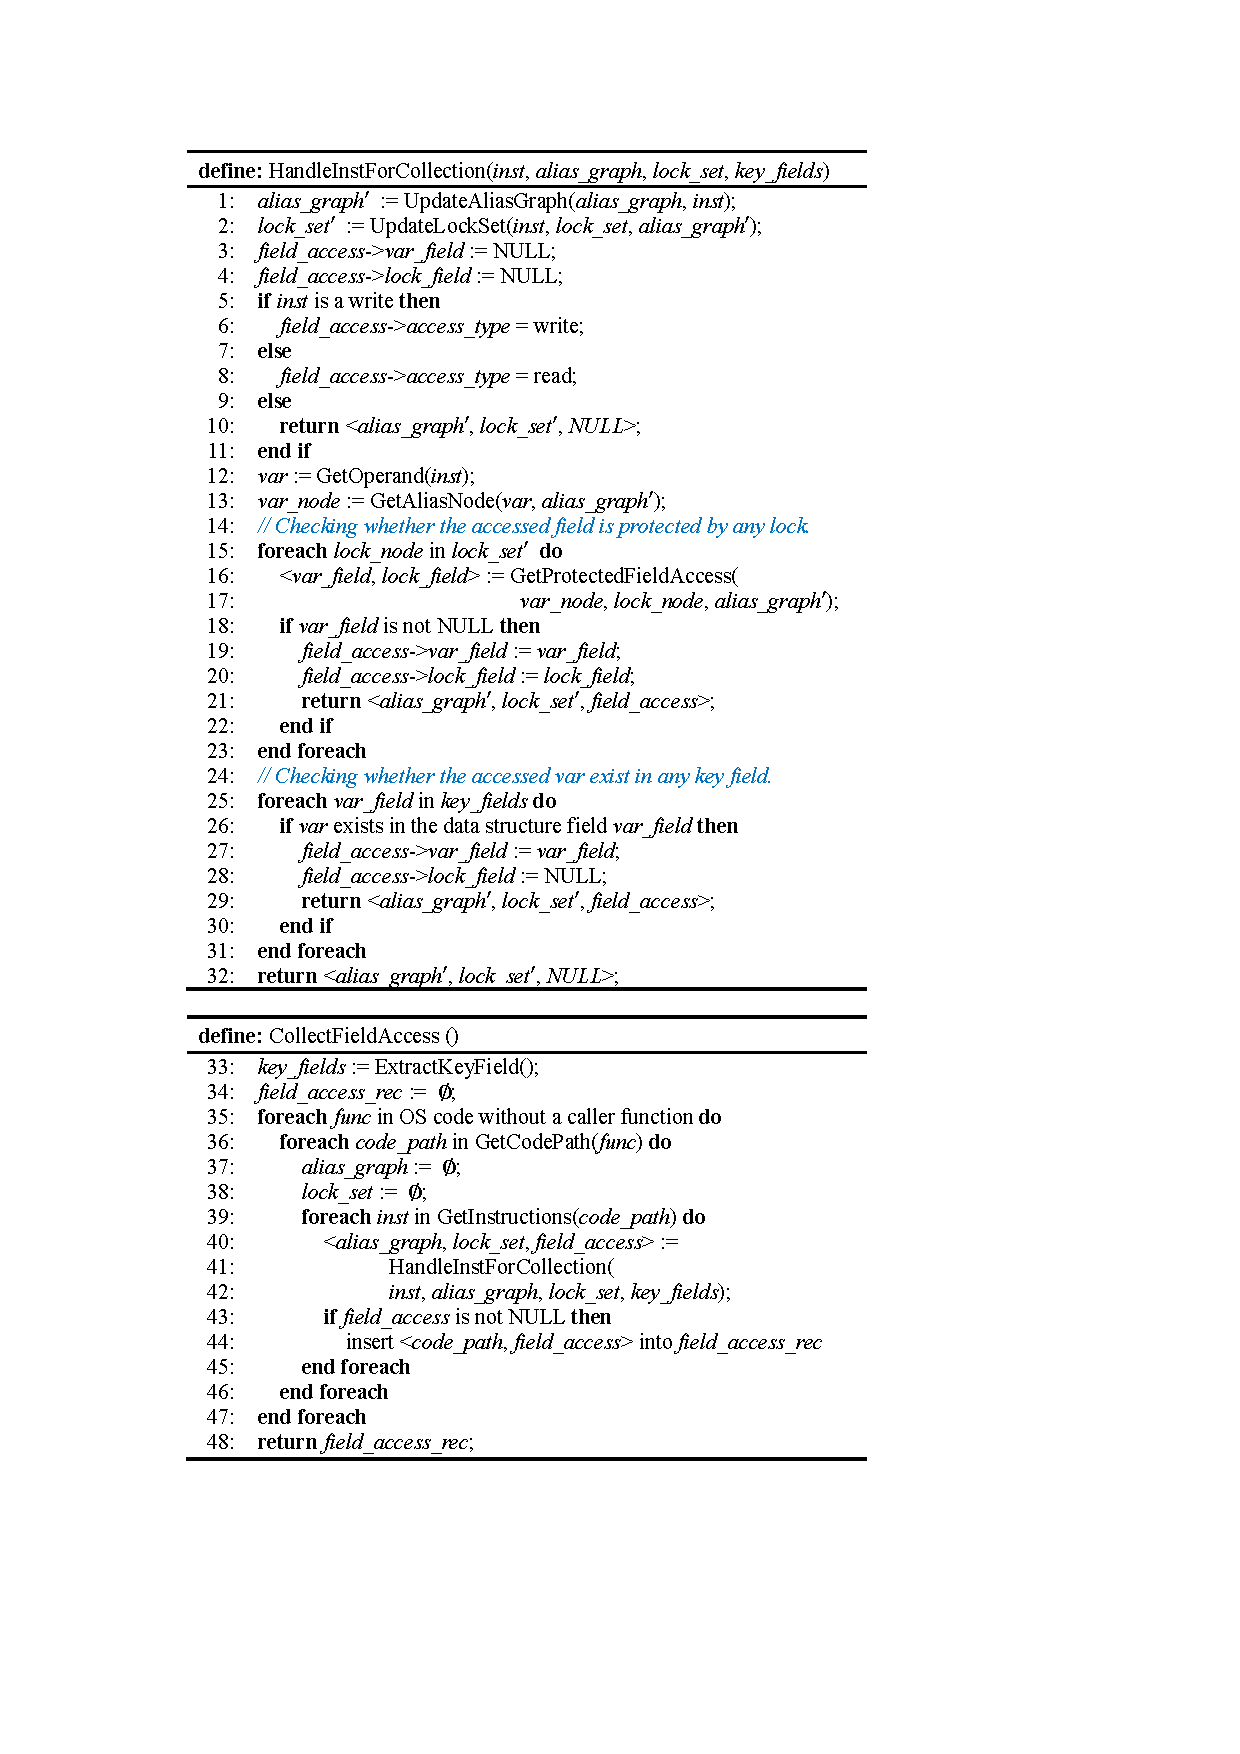
\includegraphics[width=1\linewidth]{figures/fig_pseudocode_access_collect.pdf}
	\figcaption{Pseudocodes of key-field extraction.}
	\label{fig_pseudocode_access_collect}
\end{figure}

Figure~\ref{fig_pseudocode_access_collect} shows the pseudocode to collect all 
accesses to key fields. Similarly to the key-field extraction, this stage also 
performs a path-based analysis. For each instruction in the code path (Lines 
39-45), the analysis first updates the alias graph and the lock set according 
to the handled instruction (Lines 1-2). And then, the access type (either a 
write or a read) is set according to the instruction (Lines 5-8). However, if 
the instruction is not an access operation, the function returns a NULL value 
for the field access (Line 10). Otherwise, the analysis first gets the node of 
the operand with the new alias graph (Lines 12-13), and then for each node of 
the lock variable in the lock set, the analysis uses the alias graph to extract 
the fields that the accessed variable and the lock variable stored in (Lines 
16-17). If the fields are found, the field access is returned with the found 
fields (Lines 18-22). If the fields are not found, the accessed variable  are 
not protected by any lock. In this case, if the accessed variable is stored in 
a key field, the field access is returned with a NULL lock variable (Lines 
25-30).

\PP{S3: Locking-rule deduction.} After collecting all accesses to key fields, 
the analysis deduces locking rules based on statistics. However, on the one 
hand, distinguishing different accesses to the same data structure field by 
different program sites is not fine-grained enough, because the access to a 
variable and the acquirement to a specific lock are often packaged in a special 
function, and all accesses under different calling context are regarded as the 
same access. On the other hand, distinguishing different accesses by different 
code paths can also suffer from inaccuracy when a function contains many branch 
statement and cause numerous code paths for the same variable access. Based on 
this consideration, the analysis distinguishes different accesses to the same 
data structure field by different calling contexts. Specifically, given a key 
field {\em f} and a lock {\em l}, the analysis first finds all access to {\em 
f} with lock {\em l} from the collected field accesses in Stage 2, and gets the 
number {\em locked\_access\_num} by counting different calling contexts 
extracted from the code paths of these field accesses. Then, the analysis finds 
all access to {\em f} (no matter which lock is accessed), and gets the number 
{\em all\_access\_num} in the same way as {\em locked\_access\_num}. If the 
ratio {\em locked\_access\_num}/{\em all\_access\_num} is larger than a given 
threshold, and there is at least one write access to {\em f}, the data 
structure field {\em f} is inferred to be protected by the lock {\em l}. After 
deducting locking rules, the analysis detects data races by checking whether a 
field access validates any locking rules.

\begin{figure}[htbp]
	\centering
	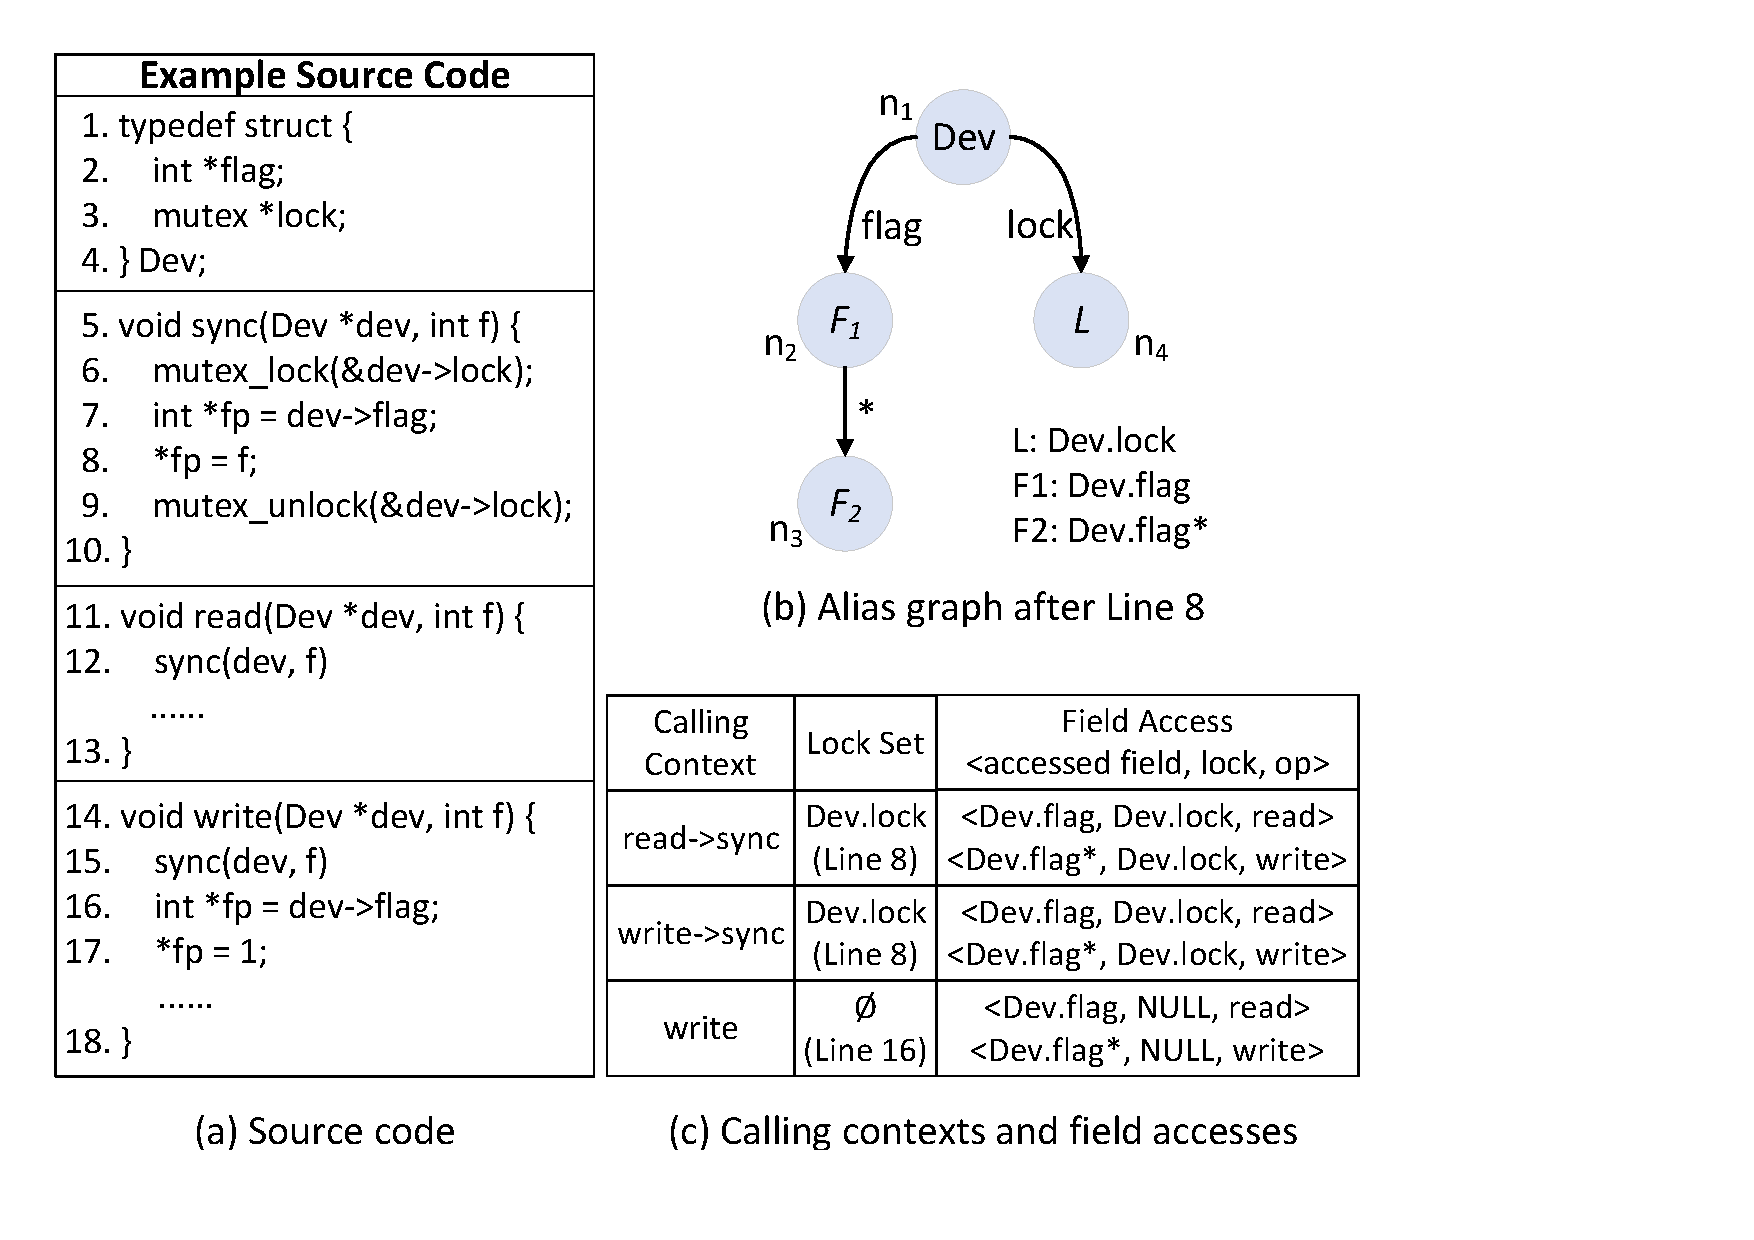
\includegraphics[width=1\linewidth]{figures/fig_demo_rule_mining.pdf}
	\figcaption{Example of locking-rule mining.}
	\label{fig_demo_rule_mining}
\end{figure}

\noindent{\textbf{\em Example.}} We use an example in 
Figure~\ref{fig_demo_rule_mining} to illustrate how to mine locking rules 
with the three stages. The analysis first performs a path-based analysis to 
extract key fields. Take the code path {\tt Line 12, Line 6, Line 7, Line 8, 
Line 9} as an example. The analysis updates the alias graph by handling two GEP 
operations ({\em \&dev->lock} and {\em fp = dev->flag}) and a STORE operation 
({\em *fp = f}). The final alias graph is shown in 
Figure~\ref{fig_demo_rule_mining}(b). At the same time as alias analysis, the 
analysis records the acquired lock {\em Dev.lock} into the lock set after the 
lock instruction at Line 6. When analyzing the read instruction at Line 7, the 
analysis finds the node of the accessed field ($\mathit{n_2}$) and the node of 
the lock stored in the lock set ($\mathit{n_4}$) has the same ancestor 
($\mathit{n_1}$), and thus {\em Dev.flag} is a key field. Similarly, {\em 
Dev.flag*} is also a key field, due to the write instruction at Line 8. 

After extracting key fields, the method collects all accesses to key fields 
with lock set analysis and the alias graph. Take the code path {\tt Line 15, 
Line 6, Line 7, Line 8, Line 9, Line 16 and Line 17} as an example, through a 
lock instruction at Line 6, the analysis records the acquired lock {\em 
Dev.lock} into the lock set. When analyzing the read instruction at Line 7, the 
analysis finds the node of the accessed field ($\mathit{n_2}$) and the node of 
the lock stored in the lock set ($\mathit{n_4}$) has the same ancestor 
($\mathit{n_1}$), and thus records a field access <{\em Dev.flag}, {\em 
Dev.lock}>. Similar to the read instruction at Line 7, the method also records 
a field access <{\em Dev.flag*}, {\em Dev.lock}> for the write instruction at 
Line 8. Then through an unlock operation at Line 9, the analysis removes the 
lock {\em Dev.lock} from the lock set. As a result, the key fields {\em 
Dev.flag} and {\em Dev.flag*} are accessed without acquiring any lock, and thus 
the analysis records two field accesses <{\em Dev.flag}, {\em NULL}> and <{\em 
Dev.flag*}, {\em NULL}>. The final field accesses are shown in 
Figure~\ref{fig_demo_rule_mining}(c).

After collecting all field accesses, the analysis finds that the fields {\em 
Dev.flag} and {\em Dev.flag*} are accessed under three calling contexts, and 
two of them are protected by the lock {\em Dev.lock}. And thus the two fields 
{\em Dev.flag} and {\em Dev.flag*} are deduced to be protected by the lock {\em 
Dev.lock} (assume the threshold of the ratio {\em locked\_access\_num} / 
{\em all\_access\_num} is 0.6). However, the accesses at Lines 16 and 17 are 
not protected by {\em Dev.lock} and thus causing two data races.

\subsection{Lock-Usage Analysis}
\label{subsec_lock_usage_analysis}
Our analysis takes functions that have no caller function as the entry as 
existing work~\cite{Li:ASPLOS22}, and performs a path-based analysis. It 
assumes that all codes reaching from entry functions can execute concurrently 
to reduce false negatives. However, this assumption is too conservative and can 
introduce many false positives because not all entry functions can execute 
concurrently in fact. We observe that each kernel module has an initialization 
phase, after which many functions can be called concurrently by other modules. 
When performing initialization, the kernel module serially initialized the lock 
and prepare other data for subsequent operations. And thus functions with the 
lock initialization and functions called by them tend not to be executed 
concurrently. Based on the observation, we propose a lock-usage analysis to 
filter out false positives caused by code that can not execute concurrently.

\begin{figure}[htbp]
	\centering
	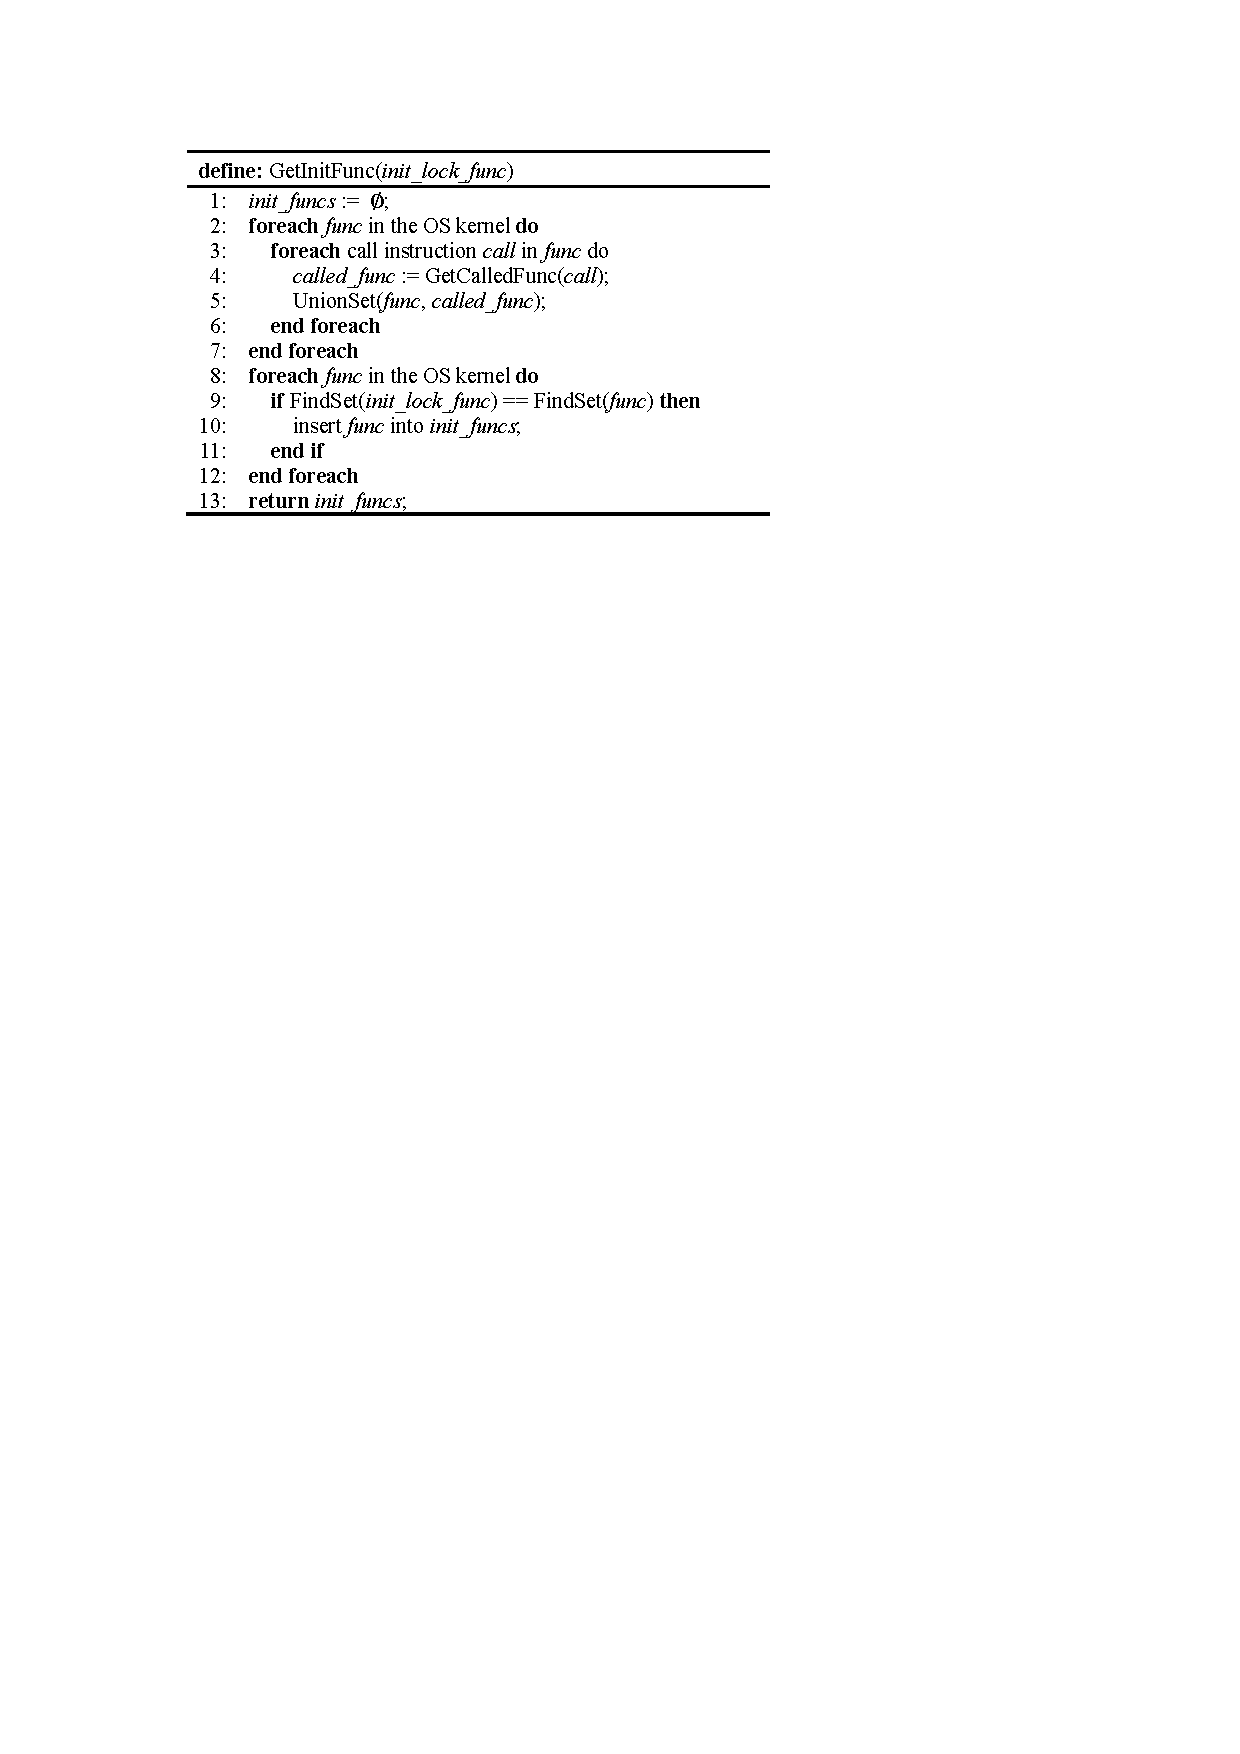
\includegraphics[width=0.9\linewidth]{figures/fig_pseudocode_lock_usage.pdf}
	\figcaption{Pseudocodes of lock-usage analysis.}
	\label{fig_pseudocode_lock_usage}
\end{figure}

Our lock-usage analysis uses the union-find set~\cite{Galler:ACM64} to get all 
functions that are reachable from the lock initialization function such as {\em 
mutex\_init()} and {\em spin\_lock\_init()}. 
Figure~\ref{fig_pseudocode_lock_usage} shows the pseudocodes of the lock-usage 
analysis. For each analyzed function in the OS kernel, the analysis first gets 
all the called functions of it (Lines 3-4), and then union the analyzed  
function and the called function to update the union-find set (Line 5). After 
processing all the call instructions, the analysis judges whether a function 
executes in the initialization phase by checking whether it exists in the same 
set with the given lock initialization function (Lines 9-11).

\begin{figure}[htbp]
	\centering
	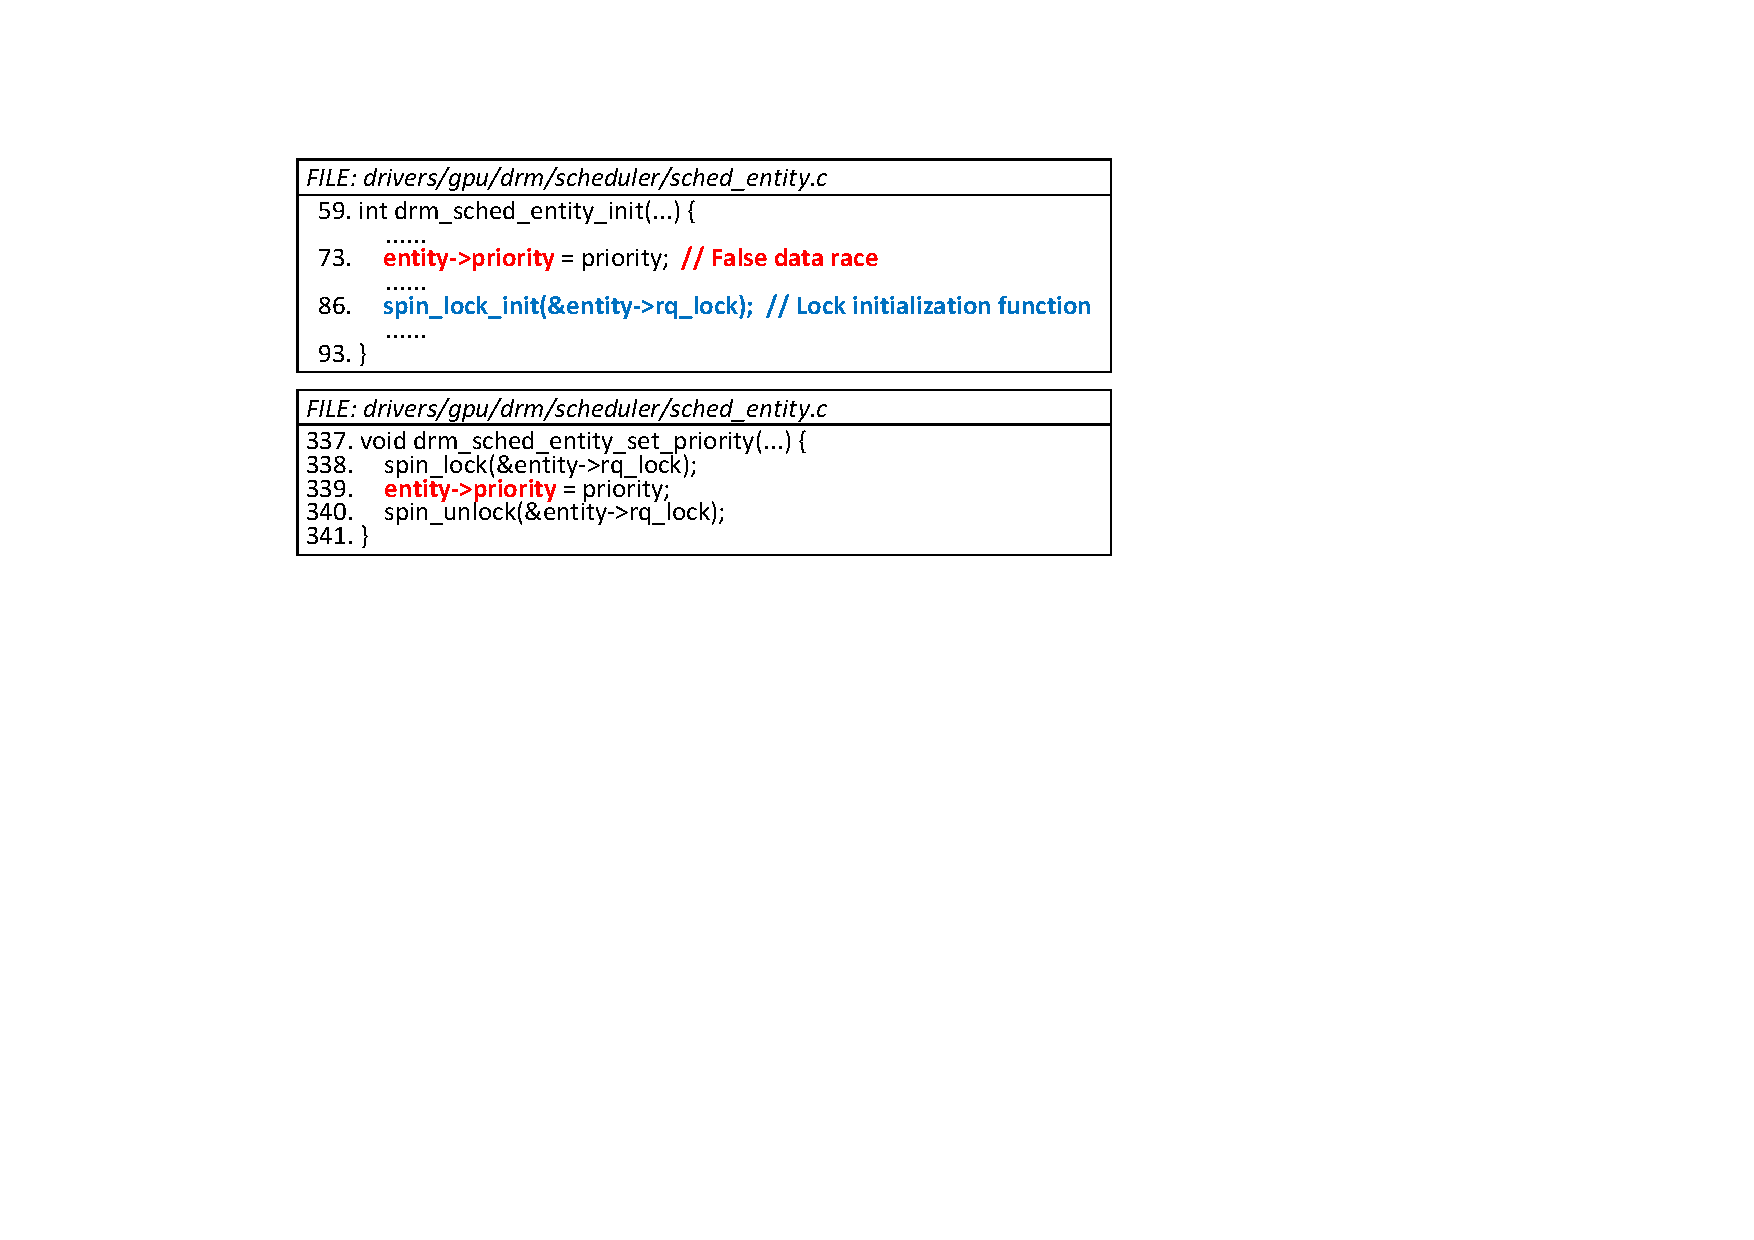
\includegraphics[width=0.9\linewidth]{figures/fig_demo_lock_usage.pdf}
	\figcaption{A false data race filtered out by our lock-usage analysis.}
	\label{fig_demo_lock_usage}
\end{figure}

\noindent{\textbf{\em Example.}} Figure~\ref{fig_demo_lock_usage} shows a false 
data race filtered out by our lock-usage analysis in the Linux DRM scheduler. 
For example in {\em drm\_sched\_entity\_set\_priority()}, the accesses to {\em 
entity->priority} is protected by the lock {\em entity->rq\_lock} in most 
cases. Therefore, {\em entity-priority} is deduced to be protected by the lock 
{\em entity->rq\_lock}. But in {\em drm\_sched\_entity\_init()}, {\em 
entity->priority} is written without acquiring the lock {\em entity->rq\_lock} 
and thus introducing a possible data race. However, the lock initialization 
function {\em spin\_lock\_init()} is called at Line 86 by {\em 
drm\_sched\_entity\_init()}. And thus {\em drm\_sched\_entity\_init()} is 
inferred to execute in the module initialization phase and can not execute 
concurrently with other functions, and this is a false data race.

\subsection{Pattern-Based Estimation}
\label{subsec_estimation}
Many data races are benign or introduced by developers deliberately to improve 
kernel performance. They can not cause memory or logic bugs, and thus 
developers are unwilling to put effort into repairing them. We observe that 
harmful data races match some typical patterns, and propose a {\em 
pattern-based estimation} to extract data races that can cause memory or logic 
bugs.

At present, we propose three patterns that can cause null-pointer dereference, 
data inconsistency and unprotected write, because these three patterns are 
common and dangerous in OSes. The three patterns are shown in 
Figure~\ref{fig_pattern}, and we assume that accesses to the fields of {\em 
dev} should be protected by {\em dev->lock}.

\begin{figure}[htbp]
	\centering
	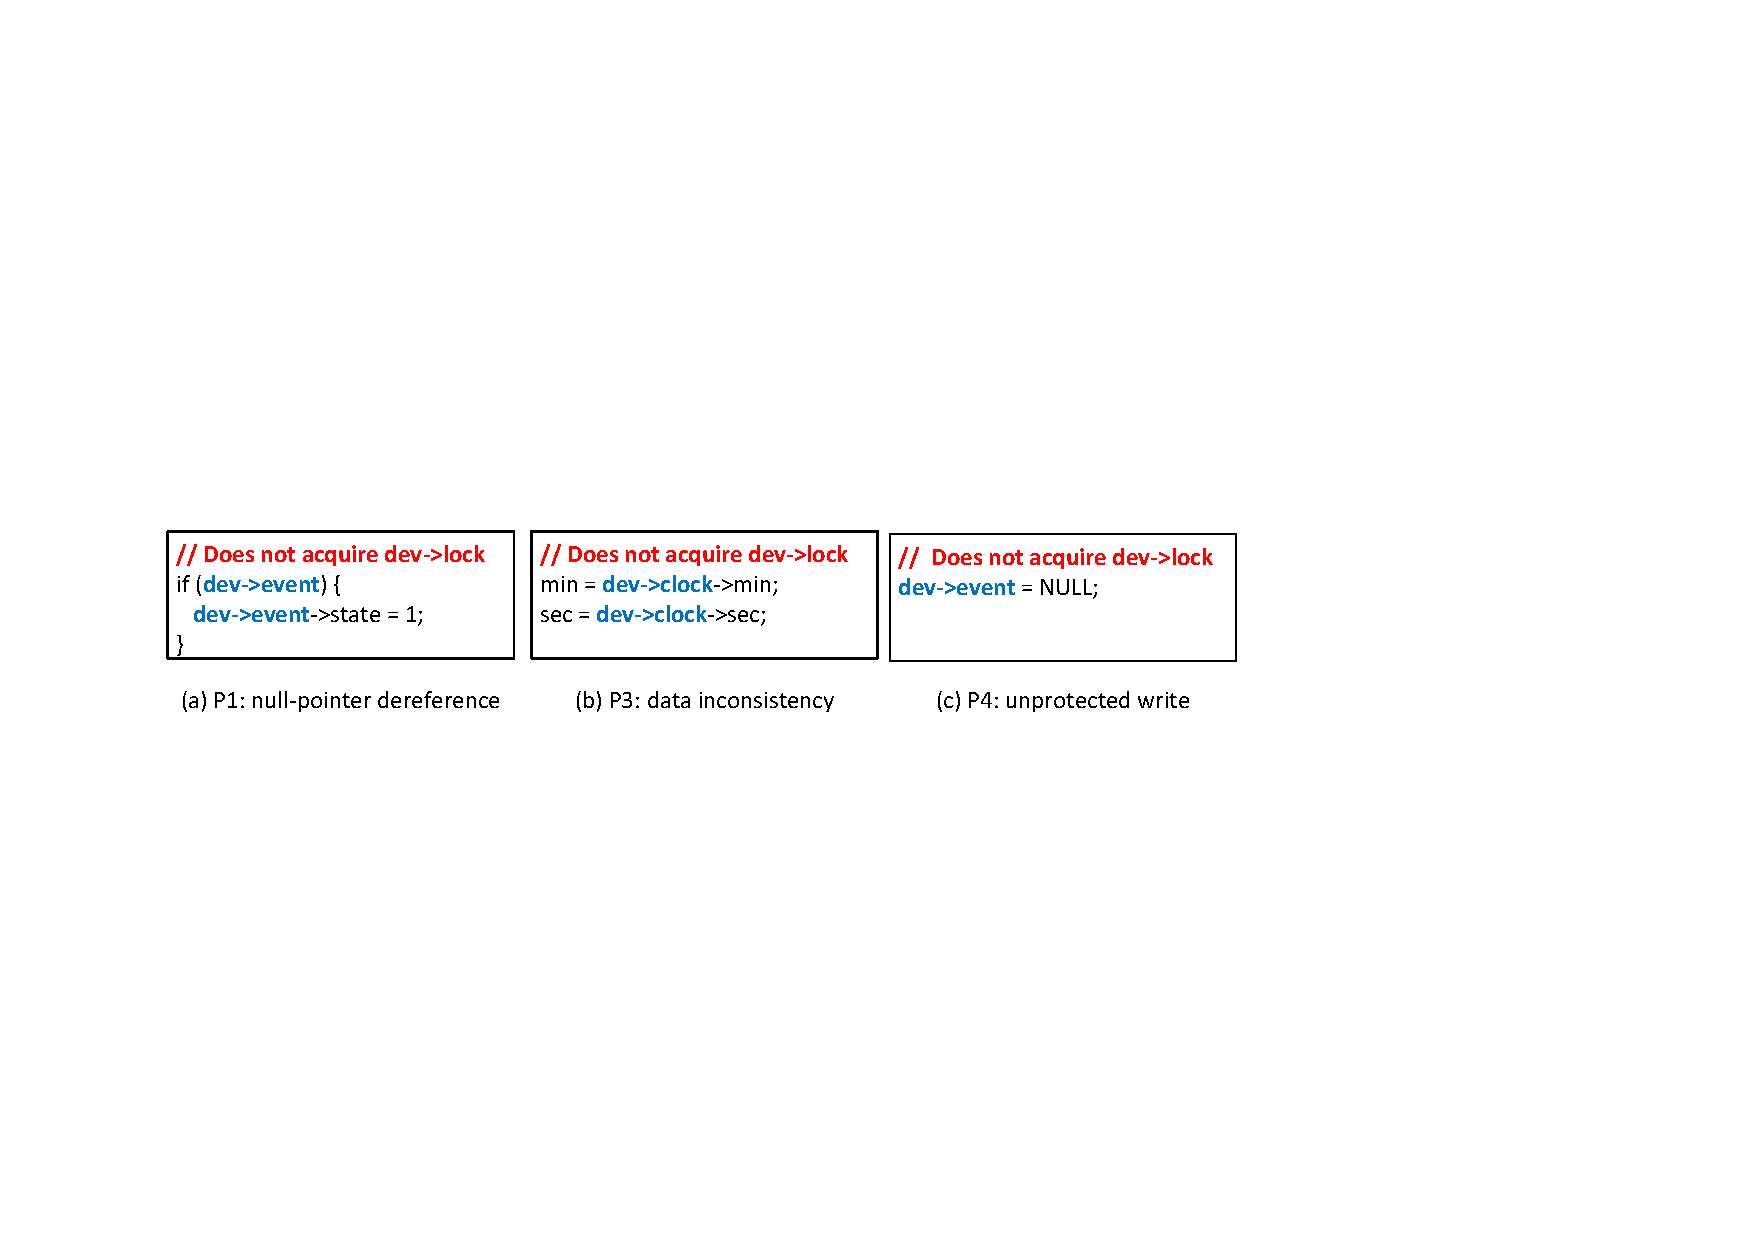
\includegraphics[width=1\linewidth]{figures/fig_pattern.pdf}
	\figcaption{Three harmful patterns of data races.}
	\label{fig_pattern}
\end{figure}

\begin{itemize}
	\item \PP{Null-pointer dereference.} The two accesses to {\em dev->event} 
	are not protected by {\em dev->lock}. This can cause a null-pointer 
	dereference if {\em dev->event} is set to NULL right after the condition of 
	the if statement is checked to be true. To recognize such a pattern, the 
	analysis first locates the data race, if it is checked by an if statement 
	and then dereferenced, a possible null-pointer dereference can occur.
	%\item \PP{Infinite loop.} The condition of the while statement does not 
	%protected by {\em dev->lock}. This can cause a infinite loop when {\em 
	%dev->cnt} is assigned with a non-zero value every time before it is 
	%checked 
	%by the while statement. The analysis detects such bugs by judge whether 
	%the 
	%data race acts as a condition of a loop statement.
	\item \PP{Data inconsistency.} Two different fields of the same data 
	structure are accessed without acquiring {\em dev->lock}. This can cause a 
	data inconsistency when the data structure field {\em dev->clock} is 
	changed by another thread right after the access to {\em dev->clock->min}. 
	To recognize such a pattern, the analysis detects whether multiple fields 
	of 	the same data structure are accessed without acquiring the protecting 
	lock.
	\item \PP{Unprotected write.} The write access to {\em dev->event} is not 
	protected by {\em dev->lock}. This is dangerous because the value {\em 
	dev->event} can be modified at any time when other threads access it, and 
	thus introduce unpredictable behavior. The analysis detects such a pattern 
	by judging whether a data race occurs in a write access.
\end{itemize}

% !TeX spellcheck = en_US
\section{\sys Approach}
\label{sec_framework}

Based on the three key techniques in Section~\ref{sec_technique}, we develop a 
practical static approach named \sys, to detect data races in OS kernels, and 
estimate harmfulness of these data races. We have implemented \sys with 
Clang~\cite{Clang} and Z3~\cite{Z3}. \sys automatically mines locking rules, 
detects data races and estimates the harmfulness of detected data races. 
Figure~\ref{fig_architecture} shows the architecture of \sys, which has four 
phases:

\begin{figure}[htbp]
	\centering
	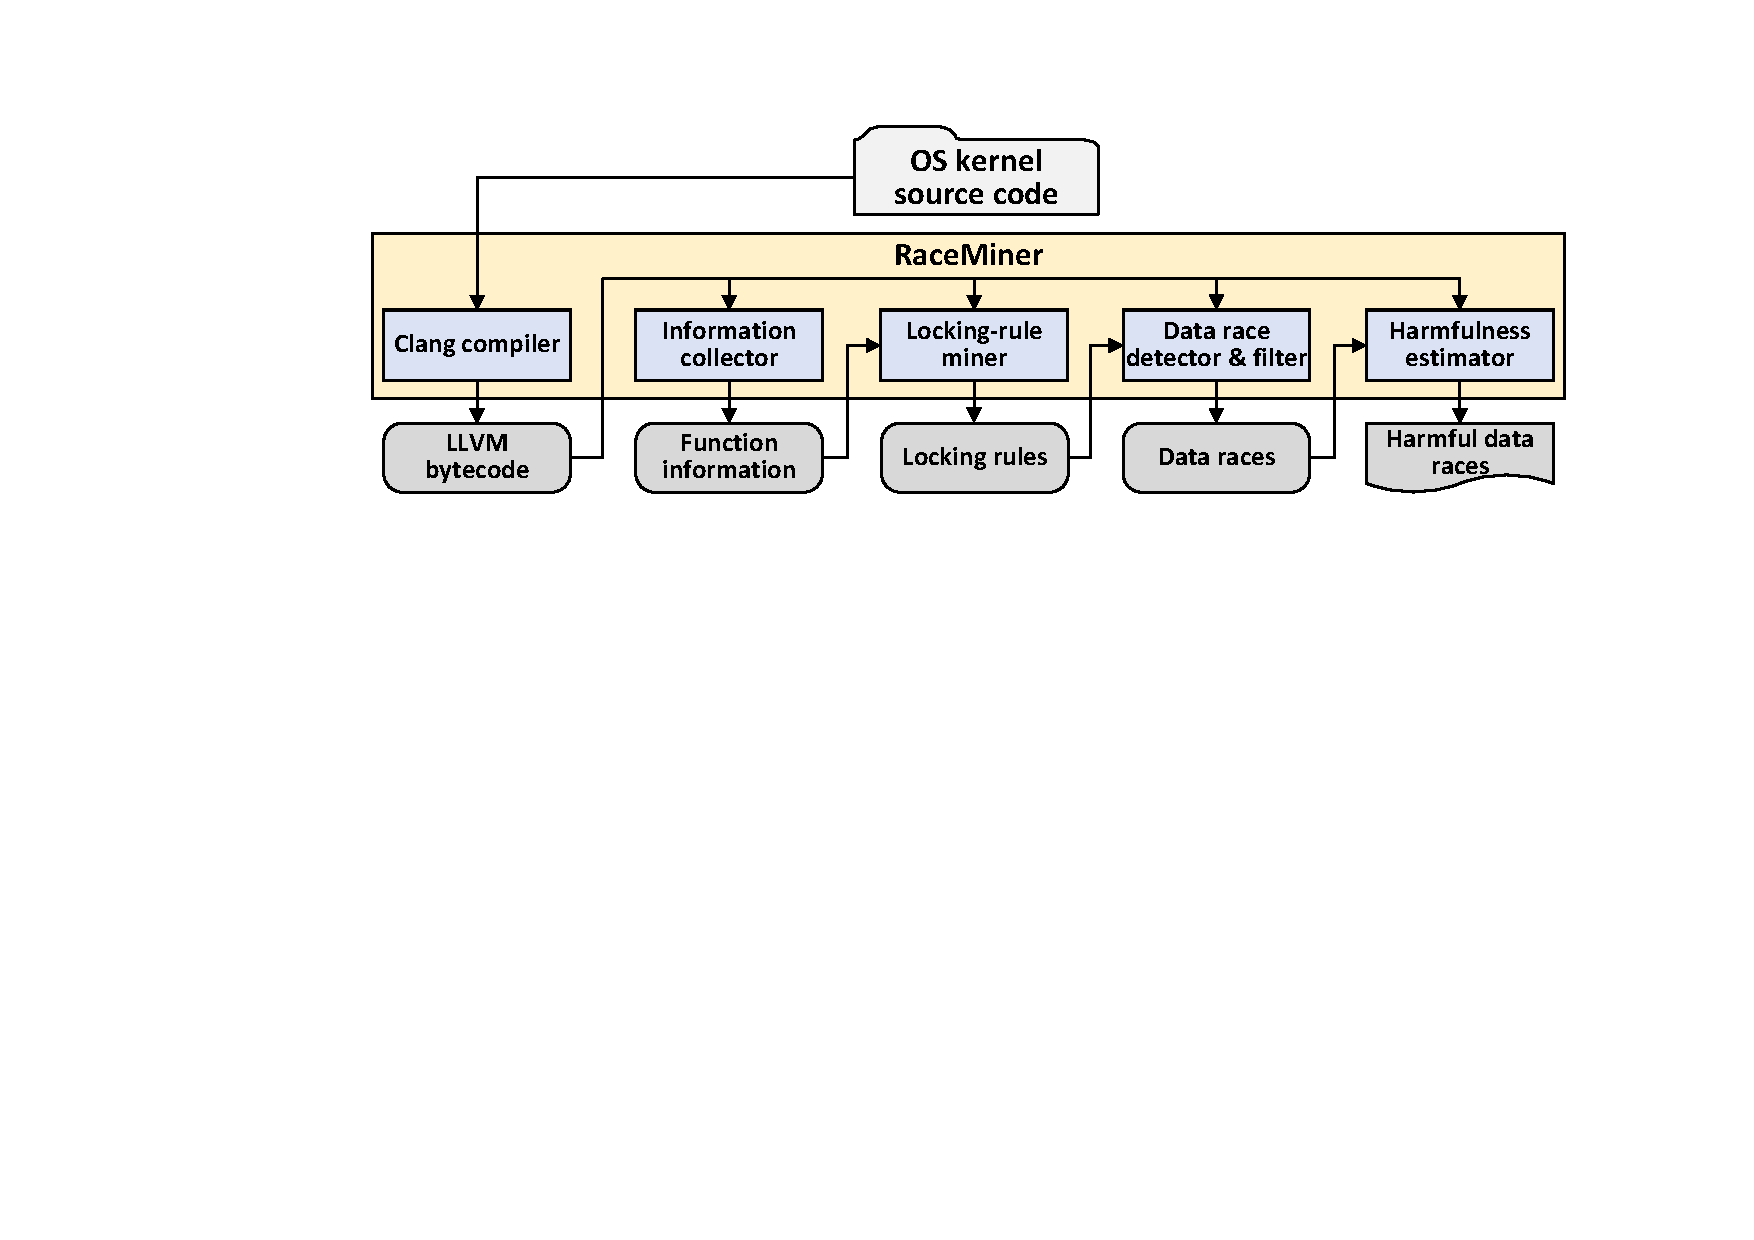
\includegraphics[width=1\linewidth]{figures/fig_architecture.pdf}
	\figcaption{\sys architecture.}
	\label{fig_architecture}
\end{figure}

\PP{P1: Source-code compilation.} The Clang compiler compiles the OS source 
code into LLVM bytecode, and then the information collector scans each LLVM 
bytecode file to record function information (including the position of each 
function definition and function name, etc.) in a database. Such information is 
used in subsequent code analysis for inter-procedural analysis across source 
files.

\PP{P2: Locking-rule Mining.} The locking-rule miner uses our alias-aware rule 
mining method to deduce locking rules about whether a variable access should be 
protected by a lock and which lock is required.

\PP{P3: Data race detection and false-positive filtering.} The data race 
detector detecting data races by checking whether a given access violate the 
rules mined by our locking-rule miner. If so, the data race filter drops 
false-positives with our locking-usage analysis. Besides, for a given data 
race, there may be multiple code paths from the entry function to its 
problematic instruction, and thus many repeated data races can be reported.  
To drop repeated data races, for a new possible data race, the data race filter 
checks whether its problematic instruction is identical to any existing data 
race. If so, this possible data race is regarded as repeated and dropped.

\PP{P4: Harmfulness estimation.} The harmfulness estimator uses our 
pattern-based estimation to estimate the harmfulness of detected data races, 
and reports data races that can cause memory or logic bugs. With these result, 
developers can focus on those harmful data races.
% !TeX spellcheck = en_US
\section{Evaluation}
\label{sec_evaluation}

To validate the effectiveness of \sys, we evaluate it on the code of Linux 
kernel 6.2. We run the evaluation on a regular x86-64 desktop with sixteen 
Intel i7-10700 CPU@2.90GHz processors and 64GB physical memory. We use the 
kernel configuration {\em allyesconfig} to enable all kernel code for the 
x86-64 architecture.

\begin{table}[tbph]
	\tablecaption{Detection results of Linux 6.2.}
	\label{tbl_bug_detection}
	\renewcommand{\arraystretch}{1}
	\setlength\tabcolsep{2pt}
	\noindent{\scriptsize
		\begin{center}
			\begin{tabular}{p{1.5cm}|l|c}
				\hline
				\multicolumn{2}{c|}{\textbf{Description}} & \textbf{\sys}  
				\\ \hline
				\multirow{2}{1.5cm}{\textbf{{\em Code analysis}}} & 
				Source files (analyzed/all) & xxxK/xxxK
				\\ \cline{2-3}
				& Source code lines (analyzed/all) & xxxM/xxxM 
				\\ \cline{2-3}
				\hline
				\multirow{3}{1.5cm}{\textbf{{\em Locking-rule mining}}} & 
				Key fields / total variables& 
				\\ \cline{2-3}
				& Mined locking rules &
				\\ \cline{2-3}
				& Protected field accesses / all accesses & 0.6
				\\ \cline{2-3}
				\hline
				\multirow{2}{1.5cm}{\textbf{{\em Data race detection}}} & 
				Detected data races (real / all) & 273 / 341
				\\ \cline{2-3}
				& Dropped data races by lock-usage analysis & 63
				\\ \cline{2-3}
				\hline
				\multirow{4}{1.5cm}{\textbf{{\em Data race estimation}}}
				& Null-pointer dereference (confirmed / all) & 15 / 20
				\\ \cline{2-3}
				%& Infinite loop (confirmed / all) & 0 / 1
				%\\ \cline{2-3}
				& Data inconsistency (confirmed / all) & 7 / 10
				\\ \cline{2-3}
				& Unprotected write (confirmed / all) & 10 / 57
				\\ \cline{2-3}
				& Total harmful data races (confirmed / all) & 32 / 88
				\\ \cline{2-3}
				\hline
				\multirow{3}{1.5cm}{\textbf{{\em Time usage}}} & 
				Key-field extraction & 
				\\ \cline{2-3}
				& Data-race detection &
				\\ \cline{2-3}
				& Total time &
				\\ \cline{2-3}
				\hline
			\end{tabular}
	\end{center}}
\end{table}

\subsection{Bug Detection}
\label{subsec_bug_detection}

We configure \sys with common lock-acquiring/release functions (like {\tt 
spin\_lock and spin\_unlock}) to perform lock-set analysis to extract key 
fields and mine locking rules, and lock-initialization functions (like {\tt 
spin\_lock\_init}) to filter our false data races caused by code paths that 
can not execute concurrently. And then run \sys to automatically check the 
kernel source code. We manually check all the data races found by \sys, and 
Table~\ref{tbl_bug_detection} shows the results, and source code lines are 
counted by CLOC~\cite{cloc}. From the results, we have the following findings:

\PP{Code analysis.} \sys can scale to large code bases of OS kernels, and it in 
total analyze xxxM lines of code in xxxK source code files within xxx hours. 
The remaining xxxM lines of code in xxxK source files are not analyzed, as they 
are not enabled by the {\em allyesconfig} for the x86-64 architecture. We 
believe that \sys can also find more data races in other architectures with 
proper configuration.

\PP{Locking-rule mining.} An OS kernel has a large code base with numerous 
variables. Handling all variables when mining locking rules can introduce much 
overhead. However, we observe that a variable tend to be protected by the lock 
stored in the same data structure as the accessed variable. Based on this 
observation, our locking-rule mining method first extract a key field by 
finding whether there exists any access to it that is protected by a lock 
stored in the same data structure. This method drops xxx\% variables (xxx out 
xxx) that need to handled when mining locking rules, and thus can reduce 
overhead significantly. After extracting key fields, our locking-rule mining 
method collect all accessed to these key fields, and then deducing locking-rule 
based on statistic. In this paper, given a data structure field, we set the 
threshold of the ratio of accesses protected by a specific lock to all accesses 
to 0.6. Our alias-aware rule mining method can drop many false rules and thus 
only mines xxx rules, which can effectively reduce false data races.

\PP{Data race detection.} \sys reports 341 data races in the kernel source 
code. We spent 15 hours on checking these data races and identify that 273 of 
them are real, with a false positive rate of 19.9\%. Besides, our lock-usage 
analysis drops 63 false data races and the results shows that it can reduce 
false positives significantly.

\PP{Data race estimation.} Many data races are benign and can not cause memory 
or logic bugs, and thus developers are unwilling to put effort into repairing 
them. We exploit three patterns to detect null-pointer dereferences, data 
inconsistency and unprotected write as introduced in 
Section~\ref{subsec_estimation}, and find 88 data races in these patterns. We 
report them to developers and 32 of them have been confirmed and fixed by them. 
We still wait for response of other data races. Moreover, one of the developers 
wonders if \sys can be used in their CI to detect these problems. 
The results show that our pattern-based estimation can extract harmful data 
races effectively, and can considerably reduce the workload of developers.

\subsection{False Positives and Negatives}
\label{subsec_false_pos_neg}
\PP{False positives.} \sys reports 68 false data races, and through manually 
checking these false data races, we find that they are introduced for three 
main reasons:

First, \sys employs an alias-aware rule mining method to deduce locking rules. 
To improve the precision of mined rules, it assumes that the accessed variable 
and the protecting lock are stored in the same data structure. Even so, \sys 
can also deduce some false rules because some developers does not use locks 
properly. They take a lock/unlock pair to protect accesses to all fields in the 
same data structure, instead of the exact field should be protected for 
convenience. As a result, our alias-aware rule mining method infers that 
accesses to all fields surrounded by the lock/unlock pair should be protected 
by the lock. This reason causes \sys to report 47 false data races.

\begin{figure}[htbp]
	\centering
	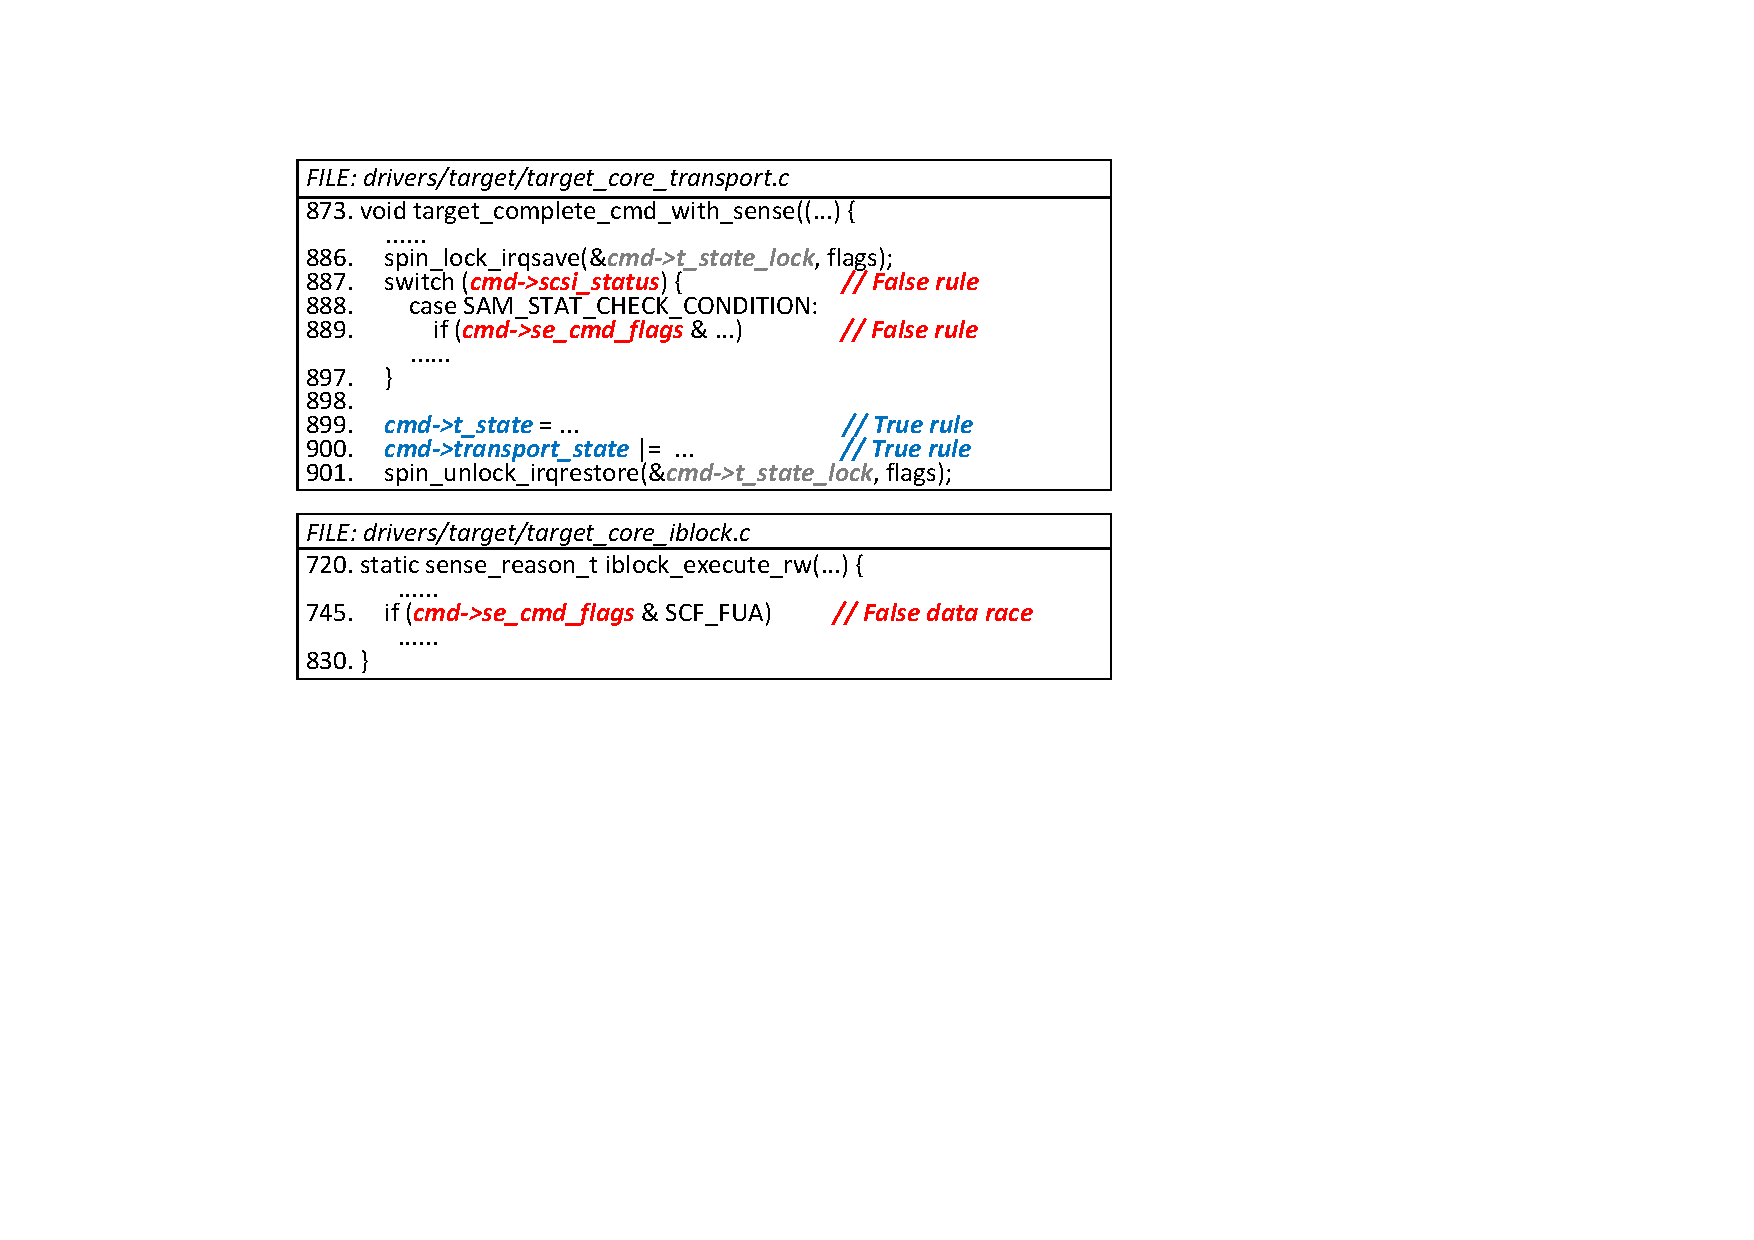
\includegraphics[width=1\linewidth]{figures/fig_demo_false_rule.pdf}
	\figcaption{A false data race caused by an incorrect locking rule.}
	\label{fig_demo_false_rule}
\end{figure}

Figure~\ref{fig_demo_false_rule} shows a false data race caused by an incorrect 
locking rule. In this example, only accesses to {\em cmd->t\_state} and {\em 
cmd->transport\_state} should be protected by the lock {\em 
cmd->t\_state\_lock}. However, the lock operation is put ahead of the switch 
statement by developers, making our alias-aware rule mining method deduces that 
{\em cmd->scsi\_status} and {\em cmd->se\_cmd\_flags} also need to be protected 
by {\em cmd->t\_state\_lock} mistakenly. Based on this incorrect locking rule, 
\sys reports a false positive at Line 745 when {\em cmd->se\_cmd\_flags} is 
accessed in an if statement. Although this data race is a false positive, it 
can cause performance degradation because the critical zone protected by the 
lock/unlock pair should have been limited to Lines 899-900.

Second, in order to reduce memory overhead and improve the performance of data 
passing among different functions, an integer can be divided into several bit 
vectors to represent different data structure fields. However, in the LLVM 
bytecode, accesses to these vectors are divided into a LOAD operation and 
several bit operations, and thus \sys can not distinguish accesses to different 
fields and reports false data races, because not all these fields should be 
protected by a lock. This reason causes \sys to report 14 false data races.

Apart from false data races caused by the two main reasons, there are still 7 
other data races. \sys regards function without caller functions in a kernel 
module as entry function and starts analysis from these entries. However, in 4 
cases, an assertion is put at the beginning of the entry function, to guarantee 
that the required lock is held, but \sys does not consider assertions and the 
subsequent accesses are regarded as unprotected. Other 3 false data races are 
accessed with {\em READ\_ONCE} or {\em WRITE\_ONCE}, and can not cause serious 
issues.

\PP{False negatives.} \sys may still miss some real data races for three main 
reasons:

First, our alias-aware mining method only considers accessed variables and 
protecting locks that exist in the same data structure. However, on the one 
hand, some accesses to variables may be protected by a global lock in a module, 
and this lock is used to protect accesses to various variables and does 
not exist in any data structure. On the other hand, some special lock 
-acquiring/release functions (such as {\em rcu\_read\_lock} and {\em 
rcu\_read\_unlock}) does not have an argument and is not handled in an alias 
graph. Therefore, locking rules in the above two cases can be missed by our 
alias-aware mining method. As a result, data races violated these locking rules 
can not detected by \sys.

Second, \sys does not handle function-pointer calls, and thus it can not build 
complete call graphs for inter-procedural analysis. However, \sys starts 
from functions without caller functions and performs analysis along call 
graphs. And as a result, functions that are only called indirectly through 
function pointers can not be analyzed by \sys, and thus data races involving 
code reached through function-pointer calls can be missed.

Finally, \sys exploits a lock-usage analysis to filter out false data races 
caused by code paths that can not execute concurrently. Specifically, the 
lock-usage analysis extracts all functions that are reachable from the lock 
initialization functions in a call graph with the union-find set, and assumes 
that these functions can not execute concurrently. However, some functions can 
be called at multiple program sites, and some of the program sites may be not 
reachable from lock initialization functions, but data races exist in these 
functions are are all dropped by our lock-usage analysis.

\subsection{Case Studies of the Found Harmful Data Races}
\label{subsec_case_study}

Figure~\ref{fig_case_bugs} shows three data races found by \sys in Linux 6.2,
and they have been confirmed by Linux kernel developers.

\begin{figure*}[htbp]
	\centering
	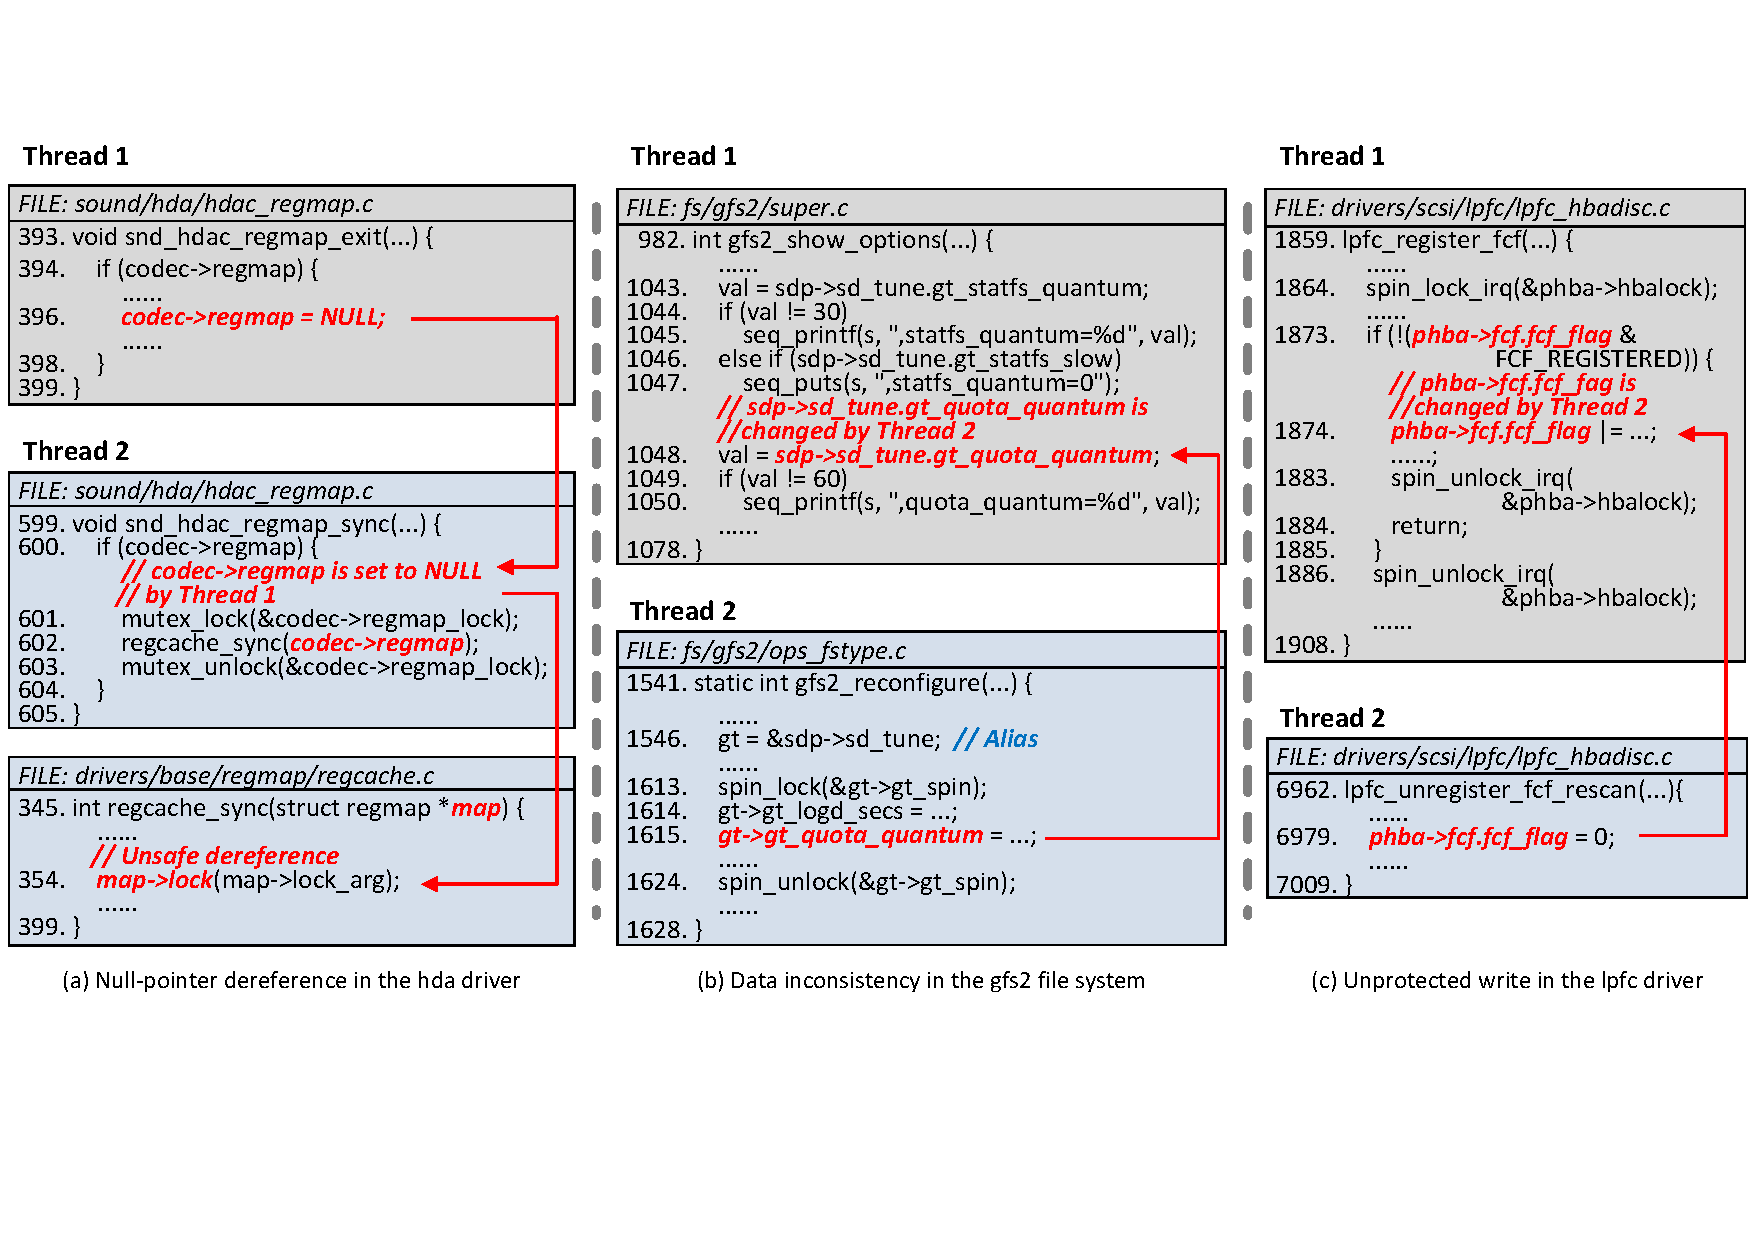
\includegraphics[width=1\linewidth]{figures/fig_case_bugs.pdf}
	\figcaption{Three real data races found by \sys in Linux 6.2.}
	\label{fig_case_bugs}
\end{figure*}

\PP{Null-pointer dereference in the HDA sound driver.} In 
Figure~\ref{fig_case_bugs}(a), the functions {\em snd\_hdac\_regmap\_exit()} 
and {\em snd\_hdac\_regmap\_sync()} can execute concurrently. In Thread 2, the 
variable {\em codec->regmap} is checked by an if statement in the function {\em 
snd\_hdac\_regmap\_sync()}. Right after the condition of the if statement is 
calculated to be true, the variable {\em codec->regmap} is set to be NULL by 
the function {\em snd\_hdac\_regmap\_exit()} in Thread 2. And then the function 
{\em regcache\_sync()} is called in Thread 1, with the argument {\em 
codec->regmap}, after acquiring the lock {\em codec->regmap\_lock}. In the 
called function, the variable {\em codec->regmap\_lock} is dereferenced through 
{\em map->lock()}. In this execution case, the data structure field {\em 
codec->regmap} is first assigned with NULL in Thread 1, and then dereferenced 
in Thread 2, and thus cause a null-pointer dereference.

\PP{Data inconsistency in the GFS2 file system.} In 
Figure~\ref{fig_case_bugs}(b), the functions {\em gfs2\_show\_options()} and 
{\em gfs2\_reconfigure()} can execute concurrently. In Thread 1, several fields 
such as {\em gt\_statfs\_quantum} and {\em gt\_quota\_quantum} of {\em 
sdp->sd\_tune} are accessed and their values are printed to logs. However, if 
the value of {\em gt->gt\_quota\_quantum} is updated by the function {\em 
gfs2\_reconfigure()} in Thread 2 right before the access to it in Thread 1, the 
values of different fields recorded in logs can be inconsistent.

\PP{Unprotected write in the LPFC SCSI driver.} In 
Figure~\ref{fig_case_bugs}(c), the value of the shared variable {\em 
phba->fcf.fcf\_flag} is set to 0 by the function {\em 
lpfc\_unregister\_fcf\_rescan()}, without acquiring the lock {\em 
phba->hbalock}, and this can cause double-fetch in several program sites. For 
example, if {\em phba->fcf.fcf\_flag} is set to 0 by Thread 2 between the two 
accesses to it in the function {\em lpfc\_register\_fcf()} in Thread 1 (Lines 
1873 and 1874), the values of the two accesses can differ, causing 
unpredictable behavior.


% !TeX spellcheck = en_US
\section{Discussion}
\label{sec_discussion}

\PP{Benefits in other aspects.} \sys uses an alias-aware mining method to 
deduce precise locking rules about whether accesses to a specific data 
structure field should be protected and which data structure field the 
protecting lock exist in. Such rules can benefit in various aspects. 

First, with these rules, developers can improve the reliability 
and performance of kernel code. On the one hand, developers can carefully check 
whether necessary locks are used when writing code, and avoid serious bugs 
caused by data races in the early developing stage. On the other hand, 
developers can limit the critical zone protected by a lock/unlock pair to the 
exact accesses that should be protected, and let other code execute 
concurrently. And these locking rules can also help improve documents of OS 
kernels, which is beneficial  for long term evolution of kernel codes.

Second, key fields extracted by \sys are data structure fields that are 
protected by some locks, and this means that these fields are likely to be 
concurrently accessed by different threads. Therefore, key fields can be used 
in detecting various types of concurrency bugs such as use-after-free and 
uninitialized-variable access. Take concurrency use-after-free as an example, 
if a key field is accessed in one thread and freed in another thread, a 
concurrency use-after-free can occur.

Finally, the locking rules deduced by our alias-aware rule mining method can 
enhance other annotation-based analyses such as Clang thread safety 
analysis~\cite{ClangThreadSafety}. Specifically, developers can use 
instrumentation to annotate necessary locks for specific variables in the code 
automatically, according to the locking rules generated by \sys, and run other 
annotation-based analysis to detect data races.

%\PP{Comparison to other approaches.} We have tried our best to experimentally 
%compare \sys to existing works in data race detection including 
%RELAY~\cite{Voung:FSE07}, WHOOP~\cite{Deligiannis:ASE15} and 
%Goblint~\cite{Vojdani:ASE16}. Unfortunately, they are too old and generate too 
%many errors when compiling and running, and thus we compare \sys to them 
%methodologically.



\PP{Limitations and future works.} \sys can be improved in some aspects. First, 
our alias-aware mining method only considers accessed variables and protecting 
locks that exist in the same data structure, and can miss some locking rules 
involving special locks such as RCU locks. To overcome this limitation, we plan 
to create a common virtual node for RCU lock in the alias graph, and regard it 
as the ancestor of all other nodes. In this way, all variables have a common 
ancestor with the RCU lock, and can be inferred to be protected by the RCU 
lock, because the accessed variable and the RCU lock are existing in the 
identical data structure in our alias-aware rule mining method. Second, \sys 
does not handle function-pointer calls, and thus it can not build complete call 
graphs, and thus can miss data races reached from function-pointer calls. To 
relieve this limitation, we plan to apply existing function-pointer 
analysis~\cite{Hind:TOPLAS99, Zhang:ISPEC15, Heintze:PLDI01} in \sys, to detect 
more data races in functions that are called through function pointers and 
reduce false negatives. Third, \sys performs a path-based analysis and suffers 
from high time overhead, to accelerate its analysis, we plan to employ 
summer-based analysis~\cite{Bai:ATC19, Bai:ATC22} to avoid re-analysis of the 
same function definition. Finally, we plan to apply \sys to detect data races 
in other OS kernels such as FreeBSD~\cite{FreeBSD} and NetBSD~\cite{NetBSD}, 
and use it to detect more types of concurrency bugs including use-after-free 
and uninitialized-variable access.
% !TeX spellcheck = en_US
\section{Related Work}
\label{sec_related}

\subsection{Static Analysis of Data Races}
\label{subsec_static}
Many approaches~\cite{Boyapati:OOPSLA02, Anderson:PLDI08, Anderson:PLDI09, 
Zhou:MICRO19, Flanagan:PASTE01, Flanagan:PLDI00, Sadowski:PLATEAU14, 
ClangThreadSafety, Blackshear:OOPSLA18, Choi:PLDI02, Engler:SOSP03, 
Voung:FSE07, Pratikakis:PLDI06, Naik:PLDI06} use static analysis to detect data 
races, without running the checked program. Some of 
them~\cite{Boyapati:OOPSLA02, Anderson:PLDI08, Anderson:PLDI09, Zhou:MICRO19, 
Flanagan:PASTE01, Flanagan:PLDI00, Sadowski:PLATEAU14, ClangThreadSafety} 
perform annotation-based analysis, and request developers to provide locking 
rules about which lock is required when a specific variable is accessed, and 
then detect data races that violate the provided rules. Clang thread safety 
analysis~\cite{ClangThreadSafety} needs developers to annotate code with a {\tt 
GUARDED\_BY} attribute to indicate which lock is required for a specific 
variable, and then works like a type system for multi-threaded 
programs~\cite{Vu:SoICT12, Boyapati:OOPSLA02, Marion:TAMC14} to detect data 
races that violate the provided attribute. Flanagan et 
al.~\cite{Flanagan:PLDI00} design a type system and rely on developers to 
provide additional type annotations to associate a protecting lock with each 
field declaration, and track the set of locks held at each program point. And 
then it identifies whether a given program is race free by checking whether 
necessary locks are indeed held at each program site. However, such 
annotation-based approaches are not suitable for race detection in OS kernels, 
because even an expert developer can not provide accurate annotations, because 
the locking rules of kernel code are not well documented, and the logic of 
kernel code tends to be very complex. Other 
approaches~\cite{Blackshear:OOPSLA18, Choi:PLDI02, Engler:SOSP03, Voung:FSE07, 
Pratikakis:PLDI06, Naik:PLDI06} employ lockset-based analysis to detect data 
races automatically. They deduce locking rules based on statistics instead of 
relying on manual annotations. But they do not consider alias 
relationships~\cite{Voung:FSE07, Engler:SOSP03} or just employ imprecise 
flow-insensitive alias analysis~\cite{Choi:PLDI02, 	Pratikakis:PLDI06, 
Naik:PLDI06}. RacerX~\cite{Engler:SOSP03} performs a lockset analysis to detect 
data races in three modes, including simple checking, simple statistical and 
precise statistical from least to most precise. However, even if for the most 
precise mode, RacerX does not employ any alias analysis, and thus introduces 
many false positives and negatives.

Different from the above static analysis, \sys employs the alias graph to mine 
locking rules automatically. Benefiting from the path-based and field-sensitive 
alias relationships generated by alias graphs, \sys can deduce locking rules 
effectively. With these locking rules, \sys can detect data races accurately. 
Moreover, \sys exploits a pattern-based estimation to extract harmful data 
races automatically, and can help developers focus on data races that can 
indeed introduce serious issues.

\subsection{Dynamic Analysis of Data Races}
\label{subsec_dynamic}
The runtime analysis does not suffer from the pointer alias problems, and thus 
many approaches~\cite{Lochmann:EuroSys19, Lu:SOSP07, Lu:FSE18, Joshi:ASE08, 	
Liu:NSDI07, Ocallahan:PPoPP03, Serebryany:WBIA09, Marino:PLDI09} detects data 
races through dynamic analysis. LockDoc~\cite{Lochmann:EuroSys19} records 
accesses to variables and lock acquisitions of an instrumented Linux kernel in 
logs, and then infers locking rules from the logs. After that, LockDoc 
automatically detect data races by checking whether a given variable access 
violates the inferred locking rules. O'callahan et al.~\cite{Ocallahan:PPoPP03} 
combine lockset-based detection and happens-before-based detection to detect 
data races, which can get fewer false positives and less overhead than previous 
dynamic analyses. In order to reduce runtime overhead further, 
LiteRace~\cite{Marino:PLDI09} employs a sampling-based approach based on the 
hypothesis that data races are likely to occur when a thread is executing
an infrequently accessed region in the program. It instruments sampled memory 
accesses, and performs happens-before-based analysis to detect data races, 
according to the logs generated by the instrumentation.

However, dynamic analysis suffers from low code coverage, and thus the locking 
rules inferred through logs can be imprecise. Besides, dynamic analyses need to 
run OS kernels with instrumentation and are hard to deploy.



% !TeX spellcheck = en_US
\section{Conclusion}
\label{sec_conclusion}

In this paper, we develop a novel static approach named \sys to detect data 
races in OS kernels by mining locking rules. It consists of three key 
techniques, including an alias-aware rule mining method to automatically deduce 
locking rules, a lock-usage analysis to filter out false positives caused by 
code paths that can not execute concurrently and a pattern-based estimation to 
extract harmful data races that can trigger memory or logical bugs such as 
null-pointer dereferences and data inconsistency. In the evaluation, \sys finds 
88 real harmful data races, and 32 of them have been confirmed by the 
developers.

\footnotesize
\bibliographystyle{plain}
\bibliography{references}


\end{document}

